\documentclass[twoside]{book}

% Packages required by doxygen
\usepackage{fixltx2e}
\usepackage{calc}
\usepackage{doxygen}
\usepackage[export]{adjustbox} % also loads graphicx
\usepackage{graphicx}
\usepackage[utf8]{inputenc}
\usepackage{makeidx}
\usepackage{multicol}
\usepackage{multirow}
\PassOptionsToPackage{warn}{textcomp}
\usepackage{textcomp}
\usepackage[nointegrals]{wasysym}
\usepackage[table]{xcolor}

% Font selection
\usepackage[T1]{fontenc}
\usepackage[scaled=.90]{helvet}
\usepackage{courier}
\usepackage{amssymb}
\usepackage{sectsty}
\renewcommand{\familydefault}{\sfdefault}
\allsectionsfont{%
  \fontseries{bc}\selectfont%
  \color{darkgray}%
}
\renewcommand{\DoxyLabelFont}{%
  \fontseries{bc}\selectfont%
  \color{darkgray}%
}
\newcommand{\+}{\discretionary{\mbox{\scriptsize$\hookleftarrow$}}{}{}}

% Page & text layout
\usepackage{geometry}
\geometry{%
  a4paper,%
  top=2.5cm,%
  bottom=2.5cm,%
  left=2.5cm,%
  right=2.5cm%
}
\tolerance=750
\hfuzz=15pt
\hbadness=750
\setlength{\emergencystretch}{15pt}
\setlength{\parindent}{0cm}
\setlength{\parskip}{3ex plus 2ex minus 2ex}
\makeatletter
\renewcommand{\paragraph}{%
  \@startsection{paragraph}{4}{0ex}{-1.0ex}{1.0ex}{%
    \normalfont\normalsize\bfseries\SS@parafont%
  }%
}
\renewcommand{\subparagraph}{%
  \@startsection{subparagraph}{5}{0ex}{-1.0ex}{1.0ex}{%
    \normalfont\normalsize\bfseries\SS@subparafont%
  }%
}
\makeatother

% Headers & footers
\usepackage{fancyhdr}
\pagestyle{fancyplain}
\fancyhead[LE]{\fancyplain{}{\bfseries\thepage}}
\fancyhead[CE]{\fancyplain{}{}}
\fancyhead[RE]{\fancyplain{}{\bfseries\leftmark}}
\fancyhead[LO]{\fancyplain{}{\bfseries\rightmark}}
\fancyhead[CO]{\fancyplain{}{}}
\fancyhead[RO]{\fancyplain{}{\bfseries\thepage}}
\fancyfoot[LE]{\fancyplain{}{}}
\fancyfoot[CE]{\fancyplain{}{}}
\fancyfoot[RE]{\fancyplain{}{\bfseries\scriptsize Generated by Doxygen }}
\fancyfoot[LO]{\fancyplain{}{\bfseries\scriptsize Generated by Doxygen }}
\fancyfoot[CO]{\fancyplain{}{}}
\fancyfoot[RO]{\fancyplain{}{}}
\renewcommand{\footrulewidth}{0.4pt}
\renewcommand{\chaptermark}[1]{%
  \markboth{#1}{}%
}
\renewcommand{\sectionmark}[1]{%
  \markright{\thesection\ #1}%
}

% Indices & bibliography
\usepackage{natbib}
\usepackage[titles]{tocloft}
\setcounter{tocdepth}{3}
\setcounter{secnumdepth}{5}
\makeindex

% Hyperlinks (required, but should be loaded last)
\usepackage{ifpdf}
\ifpdf
  \usepackage[pdftex,pagebackref=true]{hyperref}
\else
  \usepackage[ps2pdf,pagebackref=true]{hyperref}
\fi
\hypersetup{%
  colorlinks=true,%
  linkcolor=blue,%
  citecolor=blue,%
  unicode%
}

% Custom commands
\newcommand{\clearemptydoublepage}{%
  \newpage{\pagestyle{empty}\cleardoublepage}%
}

\usepackage{caption}
\captionsetup{labelsep=space,justification=centering,font={bf},singlelinecheck=off,skip=4pt,position=top}

%===== C O N T E N T S =====

\begin{document}

% Titlepage & ToC
\hypersetup{pageanchor=false,
             bookmarksnumbered=true,
             pdfencoding=unicode
            }
\pagenumbering{roman}
\begin{titlepage}
\vspace*{7cm}
\begin{center}%
{\Large Putar }\\
\vspace*{1cm}
{\large Generated by Doxygen 1.8.11}\\
\end{center}
\end{titlepage}
\clearemptydoublepage
\tableofcontents
\clearemptydoublepage
\pagenumbering{arabic}
\hypersetup{pageanchor=true}

%--- Begin generated contents ---
\chapter{Namespace Index}
\section{Namespace List}
Here is a list of all documented namespaces with brief descriptions\+:\begin{DoxyCompactList}
\item\contentsline{section}{\hyperlink{namespaceputar}{putar} \\*Putslam name space }{\pageref{namespaceputar}}{}
\end{DoxyCompactList}

\chapter{Hierarchical Index}
\section{Class Hierarchy}
This inheritance list is sorted roughly, but not completely, alphabetically\+:\begin{DoxyCompactList}
\item \contentsline{section}{C\+L\+Parser}{\pageref{classCLParser}}{}
\item \contentsline{section}{Image\+Visualizer\+CV\+:\+:Config}{\pageref{classImageVisualizerCV_1_1Config}}{}
\item \contentsline{section}{Q\+G\+L\+Visualizer\+:\+:Config}{\pageref{classQGLVisualizer_1_1Config}}{}
\item \contentsline{section}{Hmi\+Gamepad\+:\+:Config}{\pageref{classHmiGamepad_1_1Config}}{}
\item \contentsline{section}{putar\+:\+:Hmi}{\pageref{classputar_1_1Hmi}}{}
\begin{DoxyCompactList}
\item \contentsline{section}{Hmi\+Gamepad}{\pageref{classHmiGamepad}}{}
\end{DoxyCompactList}
\item \contentsline{section}{putar\+:\+:Image\+Visualizer}{\pageref{classputar_1_1ImageVisualizer}}{}
\begin{DoxyCompactList}
\item \contentsline{section}{Image\+Visualizer\+CV}{\pageref{classImageVisualizerCV}}{}
\end{DoxyCompactList}
\item \contentsline{section}{putar\+:\+:mapcoord\+\_\+type}{\pageref{structputar_1_1mapcoord__type}}{}
\item \contentsline{section}{putar\+:\+:obj\+\_\+type}{\pageref{structputar_1_1obj__type}}{}
\item \contentsline{section}{putar\+:\+:Object3D}{\pageref{classputar_1_1Object3D}}{}
\item \contentsline{section}{putar\+:\+:Obj\+Loader}{\pageref{classputar_1_1ObjLoader}}{}
\begin{DoxyCompactList}
\item \contentsline{section}{My3ds\+Loader}{\pageref{classMy3dsLoader}}{}
\item \contentsline{section}{My\+Loader}{\pageref{classMyLoader}}{}
\end{DoxyCompactList}
\item \contentsline{section}{Observer}{\pageref{classObserver}}{}
\begin{DoxyCompactList}
\item \contentsline{section}{Q\+G\+L\+Visualizer}{\pageref{classQGLVisualizer}}{}
\end{DoxyCompactList}
\item \contentsline{section}{putar\+:\+:polygon\+\_\+type}{\pageref{structputar_1_1polygon__type}}{}
\item Q\+G\+L\+Viewer\begin{DoxyCompactList}
\item \contentsline{section}{Q\+G\+L\+Visualizer}{\pageref{classQGLVisualizer}}{}
\end{DoxyCompactList}
\item \contentsline{section}{Stopwatch$<$ TimeT, ClockT, DurationT $>$}{\pageref{classStopwatch}}{}
\item \contentsline{section}{Subject}{\pageref{classSubject}}{}
\begin{DoxyCompactList}
\item \contentsline{section}{My3ds\+Loader}{\pageref{classMy3dsLoader}}{}
\item \contentsline{section}{My\+Loader}{\pageref{classMyLoader}}{}
\end{DoxyCompactList}
\item \contentsline{section}{putar\+:\+:vertex\+\_\+type}{\pageref{structputar_1_1vertex__type}}{}
\end{DoxyCompactList}

\chapter{Class Index}
\section{Class List}
Here are the classes, structs, unions and interfaces with brief descriptions\+:\begin{DoxyCompactList}
\item\contentsline{section}{\hyperlink{classCLParser}{C\+L\+Parser} }{\pageref{classCLParser}}{}
\item\contentsline{section}{\hyperlink{classImageVisualizerCV_1_1Config}{Image\+Visualizer\+C\+V\+::\+Config} }{\pageref{classImageVisualizerCV_1_1Config}}{}
\item\contentsline{section}{\hyperlink{classQGLVisualizer_1_1Config}{Q\+G\+L\+Visualizer\+::\+Config} }{\pageref{classQGLVisualizer_1_1Config}}{}
\item\contentsline{section}{\hyperlink{classHmiGamepad_1_1Config}{Hmi\+Gamepad\+::\+Config} }{\pageref{classHmiGamepad_1_1Config}}{}
\item\contentsline{section}{\hyperlink{classputar_1_1Hmi}{putar\+::\+Hmi} }{\pageref{classputar_1_1Hmi}}{}
\item\contentsline{section}{\hyperlink{classHmiGamepad}{Hmi\+Gamepad} }{\pageref{classHmiGamepad}}{}
\item\contentsline{section}{\hyperlink{classputar_1_1ImageVisualizer}{putar\+::\+Image\+Visualizer} }{\pageref{classputar_1_1ImageVisualizer}}{}
\item\contentsline{section}{\hyperlink{classImageVisualizerCV}{Image\+Visualizer\+CV} }{\pageref{classImageVisualizerCV}}{}
\item\contentsline{section}{\hyperlink{structputar_1_1mapcoord__type}{putar\+::mapcoord\+\_\+type} }{\pageref{structputar_1_1mapcoord__type}}{}
\item\contentsline{section}{\hyperlink{classMy3dsLoader}{My3ds\+Loader} \\*Obj\+Loader implementation }{\pageref{classMy3dsLoader}}{}
\item\contentsline{section}{\hyperlink{classMyLoader}{My\+Loader} \\*Obj\+Loader implementation }{\pageref{classMyLoader}}{}
\item\contentsline{section}{\hyperlink{structputar_1_1obj__type}{putar\+::obj\+\_\+type} }{\pageref{structputar_1_1obj__type}}{}
\item\contentsline{section}{\hyperlink{classputar_1_1Object3D}{putar\+::\+Object3D} \\*3D object }{\pageref{classputar_1_1Object3D}}{}
\item\contentsline{section}{\hyperlink{classputar_1_1ObjLoader}{putar\+::\+Obj\+Loader} \\*O\+B\+J\+L\+O\+A\+D\+ER interface }{\pageref{classputar_1_1ObjLoader}}{}
\item\contentsline{section}{\hyperlink{classObserver}{Observer} }{\pageref{classObserver}}{}
\item\contentsline{section}{\hyperlink{structputar_1_1polygon__type}{putar\+::polygon\+\_\+type} }{\pageref{structputar_1_1polygon__type}}{}
\item\contentsline{section}{\hyperlink{classQGLVisualizer}{Q\+G\+L\+Visualizer} \\*Map implementation }{\pageref{classQGLVisualizer}}{}
\item\contentsline{section}{\hyperlink{classStopwatch}{Stopwatch$<$ Time\+T, Clock\+T, Duration\+T $>$} }{\pageref{classStopwatch}}{}
\item\contentsline{section}{\hyperlink{classSubject}{Subject} }{\pageref{classSubject}}{}
\item\contentsline{section}{\hyperlink{structputar_1_1vertex__type}{putar\+::vertex\+\_\+type} }{\pageref{structputar_1_1vertex__type}}{}
\end{DoxyCompactList}

\chapter{File Index}
\section{File List}
Here is a list of all documented files with brief descriptions\+:\begin{DoxyCompactList}
\item\contentsline{section}{Defs/\hyperlink{defs_8h}{defs.\+h} }{\pageref{defs_8h}}{}
\item\contentsline{section}{Defs/{\bfseries eigen3.\+h} }{\pageref{eigen3_8h}}{}
\item\contentsline{section}{Defs/{\bfseries opencv.\+h} }{\pageref{opencv_8h}}{}
\item\contentsline{section}{Defs/{\bfseries opencv\+Core.\+h} }{\pageref{opencvCore_8h}}{}
\item\contentsline{section}{H\+M\+I\+Control/\hyperlink{hmi_8h}{hmi.\+h} }{\pageref{hmi_8h}}{}
\item\contentsline{section}{H\+M\+I\+Control/{\bfseries hmi\+Gamepad.\+h} }{\pageref{hmiGamepad_8h}}{}
\item\contentsline{section}{Image\+Visualizer/{\bfseries image\+Visualizer.\+h} }{\pageref{imageVisualizer_8h}}{}
\item\contentsline{section}{Image\+Visualizer/{\bfseries image\+Visualizer\+C\+V.\+h} }{\pageref{imageVisualizerCV_8h}}{}
\item\contentsline{section}{Obj\+Loader/\hyperlink{My3dsLoader_8h}{My3ds\+Loader.\+h} }{\pageref{My3dsLoader_8h}}{}
\item\contentsline{section}{Obj\+Loader/\hyperlink{MyLoader_8h}{My\+Loader.\+h} }{\pageref{MyLoader_8h}}{}
\item\contentsline{section}{Obj\+Loader/\hyperlink{objLoader_8h}{obj\+Loader.\+h} }{\pageref{objLoader_8h}}{}
\item\contentsline{section}{Utilities/{\bfseries C\+L\+Parser.\+h} }{\pageref{CLParser_8h}}{}
\item\contentsline{section}{Utilities/{\bfseries observer.\+h} }{\pageref{observer_8h}}{}
\item\contentsline{section}{Utilities/{\bfseries stopwatch.\+h} }{\pageref{stopwatch_8h}}{}
\item\contentsline{section}{Visualizer/{\bfseries Qvisualizer.\+h} }{\pageref{Qvisualizer_8h}}{}
\end{DoxyCompactList}

\chapter{Namespace Documentation}
\hypertarget{namespaceputar}{}\section{putar Namespace Reference}
\label{namespaceputar}\index{putar@{putar}}


putslam name space  


\subsection*{Classes}
\begin{DoxyCompactItemize}
\item 
class \hyperlink{classputar_1_1Hmi}{Hmi}
\item 
class \hyperlink{classputar_1_1ImageVisualizer}{Image\+Visualizer}
\item 
struct \hyperlink{structputar_1_1mapcoord__type}{mapcoord\+\_\+type}
\item 
struct \hyperlink{structputar_1_1obj__type}{obj\+\_\+type}
\item 
class \hyperlink{classputar_1_1Object3D}{Object3D}
\begin{DoxyCompactList}\small\item\em 3D object \end{DoxyCompactList}\item 
class \hyperlink{classputar_1_1ObjLoader}{Obj\+Loader}
\begin{DoxyCompactList}\small\item\em O\+B\+J\+L\+O\+A\+D\+ER interface. \end{DoxyCompactList}\item 
struct \hyperlink{structputar_1_1polygon__type}{polygon\+\_\+type}
\item 
struct \hyperlink{structputar_1_1vertex__type}{vertex\+\_\+type}
\end{DoxyCompactItemize}
\subsection*{Typedefs}
\begin{DoxyCompactItemize}
\item 
typedef Eigen\+::\+Translation$<$ double, 3 $>$ \hyperlink{namespaceputar_a4c3cbb84a7c44d90796f404d9e2c10dc}{Vec3}\hypertarget{namespaceputar_a4c3cbb84a7c44d90796f404d9e2c10dc}{}\label{namespaceputar_a4c3cbb84a7c44d90796f404d9e2c10dc}

\begin{DoxyCompactList}\small\item\em 3 element vector class \end{DoxyCompactList}\item 
typedef Eigen\+::\+Matrix$<$ double, 3, 3 $>$ \hyperlink{namespaceputar_aee57be2241e98d794717b88483857084}{Mat33}\hypertarget{namespaceputar_aee57be2241e98d794717b88483857084}{}\label{namespaceputar_aee57be2241e98d794717b88483857084}

\begin{DoxyCompactList}\small\item\em Matrix representation of S\+O(3) group of rotations. \end{DoxyCompactList}\item 
typedef Eigen\+::\+Quaternion$<$ double $>$ \hyperlink{namespaceputar_a80c20cdfaa95579ce0f4eaf85f609e31}{Quaternion}\hypertarget{namespaceputar_a80c20cdfaa95579ce0f4eaf85f609e31}{}\label{namespaceputar_a80c20cdfaa95579ce0f4eaf85f609e31}

\begin{DoxyCompactList}\small\item\em Quaternion representation of S\+O(3) group of rotations. \end{DoxyCompactList}\item 
typedef Eigen\+::\+Transform$<$ double, 3, Eigen\+::\+Affine $>$ \hyperlink{namespaceputar_a8bf3c8025ae8f60f553a752014c9849a}{Mat34}\hypertarget{namespaceputar_a8bf3c8025ae8f60f553a752014c9849a}{}\label{namespaceputar_a8bf3c8025ae8f60f553a752014c9849a}

\begin{DoxyCompactList}\small\item\em Homogeneous representation of S\+E(3) rigid body transformations. \end{DoxyCompactList}\item 
typedef cv\+::\+Mat \hyperlink{namespaceputar_a6b914df3faf7862e1bd631536309251a}{Image}\hypertarget{namespaceputar_a6b914df3faf7862e1bd631536309251a}{}\label{namespaceputar_a6b914df3faf7862e1bd631536309251a}

\begin{DoxyCompactList}\small\item\em Image. \end{DoxyCompactList}\item 
typedef struct \hyperlink{structputar_1_1obj__type}{putar\+::obj\+\_\+type} $\ast$ {\bfseries obj\+\_\+type\+\_\+ptr}\hypertarget{namespaceputar_a5c44aa91da318ae2ead9456c2f2de2ac}{}\label{namespaceputar_a5c44aa91da318ae2ead9456c2f2de2ac}

\end{DoxyCompactItemize}
\subsection*{Functions}
\begin{DoxyCompactItemize}
\item 
\hyperlink{classputar_1_1Hmi}{Hmi} $\ast$ {\bfseries create\+My\+Hmi\+Gamepad} (void)\hypertarget{namespaceputar_a07c9551507f081f35299e738e5df0739}{}\label{namespaceputar_a07c9551507f081f35299e738e5df0739}

\item 
\hyperlink{classputar_1_1Hmi}{Hmi} $\ast$ {\bfseries create\+My\+Hmi\+Gamepad} (std\+::string config\+Filename)\hypertarget{namespaceputar_abb9a094ef84d39575e3c6c3aa6800dc4}{}\label{namespaceputar_abb9a094ef84d39575e3c6c3aa6800dc4}

\item 
\hyperlink{classputar_1_1ImageVisualizer}{Image\+Visualizer} $\ast$ {\bfseries create\+My\+Image\+Visualizer} (void)\hypertarget{namespaceputar_a83c66ec1932bded19ad6caaf5f8f3b3d}{}\label{namespaceputar_a83c66ec1932bded19ad6caaf5f8f3b3d}

\item 
\hyperlink{classputar_1_1ImageVisualizer}{Image\+Visualizer} $\ast$ {\bfseries create\+My\+Image\+Visualizer} (std\+::string config\+Filename)\hypertarget{namespaceputar_a3d9bc80f022fe9d2dd490daab1a06158}{}\label{namespaceputar_a3d9bc80f022fe9d2dd490daab1a06158}

\item 
\hyperlink{classputar_1_1ObjLoader}{Obj\+Loader} $\ast$ \hyperlink{namespaceputar_a6b76c4a83de676f506ccfb24399705fb}{create\+My3ds\+Loader} (void)\hypertarget{namespaceputar_a6b76c4a83de676f506ccfb24399705fb}{}\label{namespaceputar_a6b76c4a83de676f506ccfb24399705fb}

\begin{DoxyCompactList}\small\item\em create a single \hyperlink{classputar_1_1ObjLoader}{Obj\+Loader} \end{DoxyCompactList}\item 
\hyperlink{classputar_1_1ObjLoader}{Obj\+Loader} $\ast$ {\bfseries create\+My3ds\+Loader} (std\+::string config\+File)\hypertarget{namespaceputar_a631859f4fce1b129afd30aa34b54b728}{}\label{namespaceputar_a631859f4fce1b129afd30aa34b54b728}

\item 
\hyperlink{classputar_1_1ObjLoader}{Obj\+Loader} $\ast$ \hyperlink{namespaceputar_ad2bde0bc3257e7e3e2d8c2fa6311d42d}{create\+My\+Loader} (void)\hypertarget{namespaceputar_ad2bde0bc3257e7e3e2d8c2fa6311d42d}{}\label{namespaceputar_ad2bde0bc3257e7e3e2d8c2fa6311d42d}

\begin{DoxyCompactList}\small\item\em create a single \hyperlink{classputar_1_1ObjLoader}{Obj\+Loader} \end{DoxyCompactList}\item 
\hyperlink{classputar_1_1ObjLoader}{Obj\+Loader} $\ast$ {\bfseries create\+My\+Loader} (std\+::string config\+File)\hypertarget{namespaceputar_afcf7f746d647ed671ab7d8c0cb06e528}{}\label{namespaceputar_afcf7f746d647ed671ab7d8c0cb06e528}

\end{DoxyCompactItemize}


\subsection{Detailed Description}
putslam name space 

Adam Kaźmierczak \& Arkadiusz Bomba. 
\chapter{Class Documentation}
\hypertarget{classCLParser}{}\section{C\+L\+Parser Class Reference}
\label{classCLParser}\index{C\+L\+Parser@{C\+L\+Parser}}
\subsection*{Public Member Functions}
\begin{DoxyCompactItemize}
\item 
{\bfseries C\+L\+Parser} (int argc\+\_\+, char $\ast$argv\+\_\+\mbox{[}$\,$\mbox{]}, bool switches\+\_\+on\+\_\+=false)\hypertarget{classCLParser_a673f3bc8d1f1be44331414a1d6753869}{}\label{classCLParser_a673f3bc8d1f1be44331414a1d6753869}

\item 
std\+::string {\bfseries get\+\_\+arg} (int i)\hypertarget{classCLParser_a4496217c6d3729ca7ebadf313348829e}{}\label{classCLParser_a4496217c6d3729ca7ebadf313348829e}

\item 
std\+::string {\bfseries get\+\_\+arg} (std\+::string s)\hypertarget{classCLParser_a5ad33f45b4ce52c949a087ca3de8873f}{}\label{classCLParser_a5ad33f45b4ce52c949a087ca3de8873f}

\end{DoxyCompactItemize}


The documentation for this class was generated from the following file\+:\begin{DoxyCompactItemize}
\item 
Utilities/C\+L\+Parser.\+h\end{DoxyCompactItemize}

\hypertarget{classImageVisualizerCV_1_1Config}{}\section{Image\+Visualizer\+CV\+:\+:Config Class Reference}
\label{classImageVisualizerCV_1_1Config}\index{Image\+Visualizer\+C\+V\+::\+Config@{Image\+Visualizer\+C\+V\+::\+Config}}
\subsection*{Public Member Functions}
\begin{DoxyCompactItemize}
\item 
{\bfseries Config} (std\+::string config\+Filename)\hypertarget{classImageVisualizerCV_1_1Config_a74ef59694b51061d0a24d8ed573e6ab2}{}\label{classImageVisualizerCV_1_1Config_a74ef59694b51061d0a24d8ed573e6ab2}

\item 
void {\bfseries load} (std\+::string config\+Filename)\hypertarget{classImageVisualizerCV_1_1Config_a28ca20a9645e13ae61def6afc12600b9}{}\label{classImageVisualizerCV_1_1Config_a28ca20a9645e13ae61def6afc12600b9}

\end{DoxyCompactItemize}
\subsection*{Public Attributes}
\begin{DoxyCompactItemize}
\item 
std\+::string {\bfseries window\+Name}\hypertarget{classImageVisualizerCV_1_1Config_a8fd9eb103656339eb36fa0b1ebd5cafb}{}\label{classImageVisualizerCV_1_1Config_a8fd9eb103656339eb36fa0b1ebd5cafb}

\end{DoxyCompactItemize}


The documentation for this class was generated from the following file\+:\begin{DoxyCompactItemize}
\item 
Image\+Visualizer/image\+Visualizer\+C\+V.\+h\end{DoxyCompactItemize}

\hypertarget{classQGLVisualizer_1_1Config}{}\section{Q\+G\+L\+Visualizer\+:\+:Config Class Reference}
\label{classQGLVisualizer_1_1Config}\index{Q\+G\+L\+Visualizer\+::\+Config@{Q\+G\+L\+Visualizer\+::\+Config}}
\subsection*{Public Member Functions}
\begin{DoxyCompactItemize}
\item 
{\bfseries Config} (std\+::string config\+Filename)\hypertarget{classQGLVisualizer_1_1Config_a29d9f987c62e30900b2abb4b7c637011}{}\label{classQGLVisualizer_1_1Config_a29d9f987c62e30900b2abb4b7c637011}

\item 
void {\bfseries load} (std\+::string config\+Filename)\hypertarget{classQGLVisualizer_1_1Config_ad48e81a15ef56cd9fd723ebd982e0451}{}\label{classQGLVisualizer_1_1Config_ad48e81a15ef56cd9fd723ebd982e0451}

\end{DoxyCompactItemize}
\subsection*{Public Attributes}
\begin{DoxyCompactItemize}
\item 
bool \hyperlink{classQGLVisualizer_1_1Config_aae3376a63659789ed8a26b281c2f6f1a}{verbose}\hypertarget{classQGLVisualizer_1_1Config_aae3376a63659789ed8a26b281c2f6f1a}{}\label{classQGLVisualizer_1_1Config_aae3376a63659789ed8a26b281c2f6f1a}

\begin{DoxyCompactList}\small\item\em verbose \end{DoxyCompactList}\item 
Q\+Color \hyperlink{classQGLVisualizer_1_1Config_a6bc848665e8e4c762b295931b07ffd08}{background\+Color}\hypertarget{classQGLVisualizer_1_1Config_a6bc848665e8e4c762b295931b07ffd08}{}\label{classQGLVisualizer_1_1Config_a6bc848665e8e4c762b295931b07ffd08}

\begin{DoxyCompactList}\small\item\em Background color. \end{DoxyCompactList}\end{DoxyCompactItemize}


The documentation for this class was generated from the following file\+:\begin{DoxyCompactItemize}
\item 
Visualizer/Qvisualizer.\+h\end{DoxyCompactItemize}

\hypertarget{classHmiGamepad_1_1Config}{}\section{Hmi\+Gamepad\+:\+:Config Class Reference}
\label{classHmiGamepad_1_1Config}\index{Hmi\+Gamepad\+::\+Config@{Hmi\+Gamepad\+::\+Config}}
\subsection*{Public Member Functions}
\begin{DoxyCompactItemize}
\item 
{\bfseries Config} (std\+::string config\+Filename)\hypertarget{classHmiGamepad_1_1Config_a412a0a2eabc1a97786c94c3eb415e82c}{}\label{classHmiGamepad_1_1Config_a412a0a2eabc1a97786c94c3eb415e82c}

\item 
void {\bfseries load} (std\+::string config\+Filename)\hypertarget{classHmiGamepad_1_1Config_a9e9a34a7266583fd99a39c4e27f74c5a}{}\label{classHmiGamepad_1_1Config_a9e9a34a7266583fd99a39c4e27f74c5a}

\end{DoxyCompactItemize}
\subsection*{Public Attributes}
\begin{DoxyCompactItemize}
\item 
std\+::string \hyperlink{classHmiGamepad_1_1Config_aadc222e055ce17ba8f0dc3a8dc77c455}{devicename}\hypertarget{classHmiGamepad_1_1Config_aadc222e055ce17ba8f0dc3a8dc77c455}{}\label{classHmiGamepad_1_1Config_aadc222e055ce17ba8f0dc3a8dc77c455}

\begin{DoxyCompactList}\small\item\em devicename \end{DoxyCompactList}\item 
float \hyperlink{classHmiGamepad_1_1Config_a3c762ca0dd8a74b0ad9d4f1991b7f96b}{delay}\hypertarget{classHmiGamepad_1_1Config_a3c762ca0dd8a74b0ad9d4f1991b7f96b}{}\label{classHmiGamepad_1_1Config_a3c762ca0dd8a74b0ad9d4f1991b7f96b}

\begin{DoxyCompactList}\small\item\em delay \end{DoxyCompactList}\end{DoxyCompactItemize}


The documentation for this class was generated from the following file\+:\begin{DoxyCompactItemize}
\item 
H\+M\+I\+Control/hmi\+Gamepad.\+h\end{DoxyCompactItemize}

\hypertarget{classputar_1_1Hmi}{}\section{putar\+:\+:Hmi Class Reference}
\label{classputar_1_1Hmi}\index{putar\+::\+Hmi@{putar\+::\+Hmi}}


Inheritance diagram for putar\+:\+:Hmi\+:
\nopagebreak
\begin{figure}[H]
\begin{center}
\leavevmode
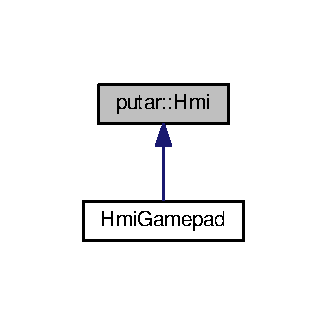
\includegraphics[width=157pt]{classputar_1_1Hmi__inherit__graph}
\end{center}
\end{figure}
\subsection*{Public Member Functions}
\begin{DoxyCompactItemize}
\item 
virtual void {\bfseries update\+Pose} (const \hyperlink{namespaceputar_a8bf3c8025ae8f60f553a752014c9849a}{Mat34} \&pose)=0\hypertarget{classputar_1_1Hmi_ab559867746b7c558c4b9370245d08ada}{}\label{classputar_1_1Hmi_ab559867746b7c558c4b9370245d08ada}

\end{DoxyCompactItemize}


The documentation for this class was generated from the following file\+:\begin{DoxyCompactItemize}
\item 
H\+M\+I\+Control/\hyperlink{hmi_8h}{hmi.\+h}\end{DoxyCompactItemize}

\hypertarget{classHmiGamepad}{}\section{Hmi\+Gamepad Class Reference}
\label{classHmiGamepad}\index{Hmi\+Gamepad@{Hmi\+Gamepad}}


Inheritance diagram for Hmi\+Gamepad\+:
\nopagebreak
\begin{figure}[H]
\begin{center}
\leavevmode
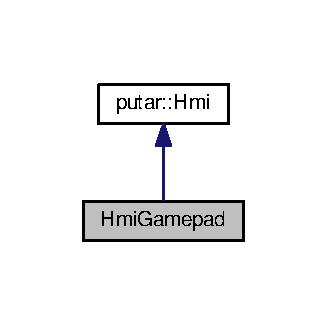
\includegraphics[width=157pt]{classHmiGamepad__inherit__graph}
\end{center}
\end{figure}


Collaboration diagram for Hmi\+Gamepad\+:
\nopagebreak
\begin{figure}[H]
\begin{center}
\leavevmode
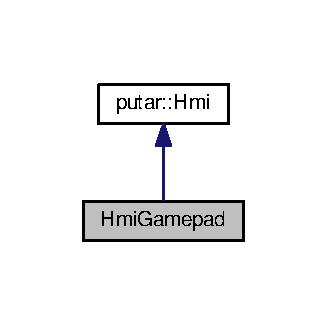
\includegraphics[width=157pt]{classHmiGamepad__coll__graph}
\end{center}
\end{figure}
\subsection*{Classes}
\begin{DoxyCompactItemize}
\item 
class \hyperlink{classHmiGamepad_1_1Config}{Config}
\end{DoxyCompactItemize}
\subsection*{Public Types}
\begin{DoxyCompactItemize}
\item 
typedef std\+::unique\+\_\+ptr$<$ \hyperlink{classHmiGamepad}{Hmi\+Gamepad} $>$ {\bfseries Ptr}\hypertarget{classHmiGamepad_a5201dddd045aaa96c7d58376c623f2cd}{}\label{classHmiGamepad_a5201dddd045aaa96c7d58376c623f2cd}

\end{DoxyCompactItemize}
\subsection*{Public Member Functions}
\begin{DoxyCompactItemize}
\item 
\hyperlink{classHmiGamepad_ae89618e8d2c7f5eccd8fd290c2ff09ab}{Hmi\+Gamepad} (std\+::string config\+Filename)\hypertarget{classHmiGamepad_ae89618e8d2c7f5eccd8fd290c2ff09ab}{}\label{classHmiGamepad_ae89618e8d2c7f5eccd8fd290c2ff09ab}

\begin{DoxyCompactList}\small\item\em Construction. \end{DoxyCompactList}\item 
void {\bfseries update\+Pose} (const \hyperlink{namespaceputar_a8bf3c8025ae8f60f553a752014c9849a}{Mat34} \&pose)\hypertarget{classHmiGamepad_ae310fd4190dfc54b15a6c54019464aa4}{}\label{classHmiGamepad_ae310fd4190dfc54b15a6c54019464aa4}

\end{DoxyCompactItemize}


The documentation for this class was generated from the following file\+:\begin{DoxyCompactItemize}
\item 
H\+M\+I\+Control/hmi\+Gamepad.\+h\end{DoxyCompactItemize}

\hypertarget{classputar_1_1ImageVisualizer}{}\section{putar\+:\+:Image\+Visualizer Class Reference}
\label{classputar_1_1ImageVisualizer}\index{putar\+::\+Image\+Visualizer@{putar\+::\+Image\+Visualizer}}


Inheritance diagram for putar\+:\+:Image\+Visualizer\+:
\nopagebreak
\begin{figure}[H]
\begin{center}
\leavevmode
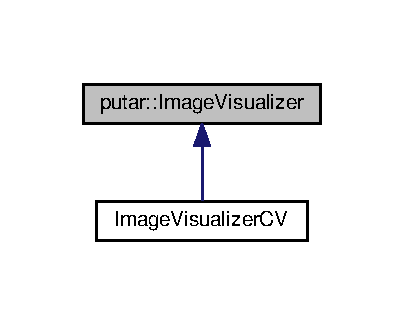
\includegraphics[width=194pt]{classputar_1_1ImageVisualizer__inherit__graph}
\end{center}
\end{figure}
\subsection*{Public Member Functions}
\begin{DoxyCompactItemize}
\item 
virtual void {\bfseries update\+Frame} (cv\+::\+Mat R\+GB, cv\+::\+Mat depth\+Img)=0\hypertarget{classputar_1_1ImageVisualizer_add122b9e49a597c121f480f57e1cb679}{}\label{classputar_1_1ImageVisualizer_add122b9e49a597c121f480f57e1cb679}

\item 
virtual void {\bfseries update\+Mask} (cv\+::\+Mat mask, cv\+::\+Mat depth\+Mask)=0\hypertarget{classputar_1_1ImageVisualizer_a2425a96f33553a34bf7c2640fff32c02}{}\label{classputar_1_1ImageVisualizer_a2425a96f33553a34bf7c2640fff32c02}

\end{DoxyCompactItemize}


The documentation for this class was generated from the following file\+:\begin{DoxyCompactItemize}
\item 
Image\+Visualizer/image\+Visualizer.\+h\end{DoxyCompactItemize}

\hypertarget{classImageVisualizerCV}{}\section{Image\+Visualizer\+CV Class Reference}
\label{classImageVisualizerCV}\index{Image\+Visualizer\+CV@{Image\+Visualizer\+CV}}


Inheritance diagram for Image\+Visualizer\+CV\+:
\nopagebreak
\begin{figure}[H]
\begin{center}
\leavevmode
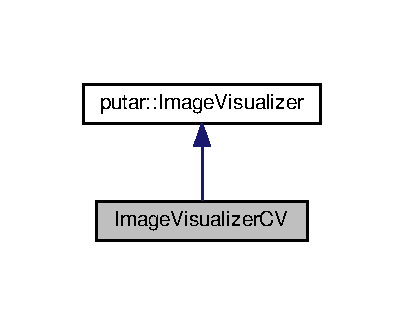
\includegraphics[width=194pt]{classImageVisualizerCV__inherit__graph}
\end{center}
\end{figure}


Collaboration diagram for Image\+Visualizer\+CV\+:
\nopagebreak
\begin{figure}[H]
\begin{center}
\leavevmode
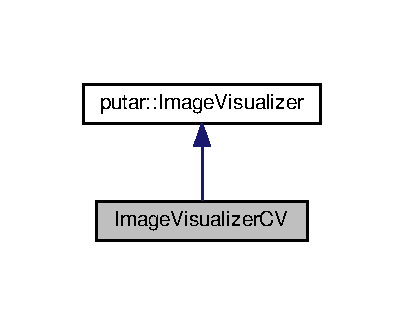
\includegraphics[width=194pt]{classImageVisualizerCV__coll__graph}
\end{center}
\end{figure}
\subsection*{Classes}
\begin{DoxyCompactItemize}
\item 
class \hyperlink{classImageVisualizerCV_1_1Config}{Config}
\end{DoxyCompactItemize}
\subsection*{Public Types}
\begin{DoxyCompactItemize}
\item 
typedef std\+::unique\+\_\+ptr$<$ \hyperlink{classImageVisualizerCV}{Image\+Visualizer\+CV} $>$ {\bfseries Ptr}\hypertarget{classImageVisualizerCV_af7f61a02a93798de851168eb425e900a}{}\label{classImageVisualizerCV_af7f61a02a93798de851168eb425e900a}

\end{DoxyCompactItemize}
\subsection*{Public Member Functions}
\begin{DoxyCompactItemize}
\item 
{\bfseries Image\+Visualizer\+CV} (std\+::string config\+Filename)\hypertarget{classImageVisualizerCV_a4adc88688d2f60c8e0d5e982a2838e79}{}\label{classImageVisualizerCV_a4adc88688d2f60c8e0d5e982a2838e79}

\item 
void {\bfseries update\+Frame} (cv\+::\+Mat R\+GB, cv\+::\+Mat depth\+Img)\hypertarget{classImageVisualizerCV_aa6c48302a07250be5fd8c988547510b7}{}\label{classImageVisualizerCV_aa6c48302a07250be5fd8c988547510b7}

\item 
void {\bfseries update\+Mask} (cv\+::\+Mat mask, cv\+::\+Mat depth\+Mask)\hypertarget{classImageVisualizerCV_a0571545cb7ac7ce7788f36d163028ee1}{}\label{classImageVisualizerCV_a0571545cb7ac7ce7788f36d163028ee1}

\end{DoxyCompactItemize}


The documentation for this class was generated from the following file\+:\begin{DoxyCompactItemize}
\item 
Image\+Visualizer/image\+Visualizer\+C\+V.\+h\end{DoxyCompactItemize}

\hypertarget{structputar_1_1mapcoord__type}{}\section{putar\+:\+:mapcoord\+\_\+type Struct Reference}
\label{structputar_1_1mapcoord__type}\index{putar\+::mapcoord\+\_\+type@{putar\+::mapcoord\+\_\+type}}
\subsection*{Public Attributes}
\begin{DoxyCompactItemize}
\item 
float {\bfseries u}\hypertarget{structputar_1_1mapcoord__type_a111e5f1af14a13716b124b5adfee16a5}{}\label{structputar_1_1mapcoord__type_a111e5f1af14a13716b124b5adfee16a5}

\item 
float {\bfseries v}\hypertarget{structputar_1_1mapcoord__type_a0625dcacb5b03d2eaf9c31bc454bfbf0}{}\label{structputar_1_1mapcoord__type_a0625dcacb5b03d2eaf9c31bc454bfbf0}

\end{DoxyCompactItemize}


The documentation for this struct was generated from the following file\+:\begin{DoxyCompactItemize}
\item 
Defs/\hyperlink{defs_8h}{defs.\+h}\end{DoxyCompactItemize}

\hypertarget{classMy3dsLoader}{}\section{My3ds\+Loader Class Reference}
\label{classMy3dsLoader}\index{My3ds\+Loader@{My3ds\+Loader}}


Obj\+Loader implementation.  




{\ttfamily \#include $<$My3ds\+Loader.\+h$>$}



Inheritance diagram for My3ds\+Loader\+:
\nopagebreak
\begin{figure}[H]
\begin{center}
\leavevmode
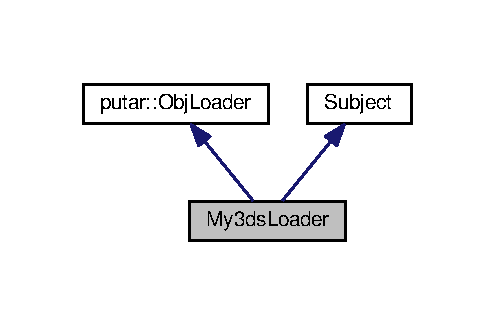
\includegraphics[width=238pt]{classMy3dsLoader__inherit__graph}
\end{center}
\end{figure}


Collaboration diagram for My3ds\+Loader\+:
\nopagebreak
\begin{figure}[H]
\begin{center}
\leavevmode
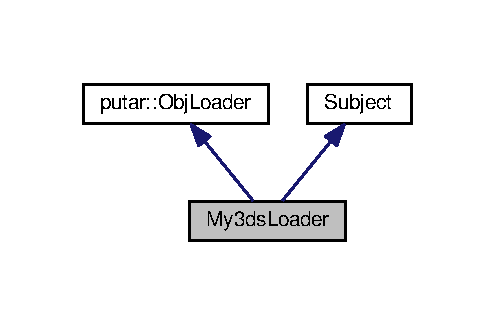
\includegraphics[width=238pt]{classMy3dsLoader__coll__graph}
\end{center}
\end{figure}
\subsection*{Public Types}
\begin{DoxyCompactItemize}
\item 
typedef std\+::unique\+\_\+ptr$<$ \hyperlink{classMy3dsLoader}{My3ds\+Loader} $>$ \hyperlink{classMy3dsLoader_a975e85ff57c2fe95a09e5c2c26377441}{Ptr}\hypertarget{classMy3dsLoader_a975e85ff57c2fe95a09e5c2c26377441}{}\label{classMy3dsLoader_a975e85ff57c2fe95a09e5c2c26377441}

\begin{DoxyCompactList}\small\item\em Pointer. \end{DoxyCompactList}\end{DoxyCompactItemize}
\subsection*{Public Member Functions}
\begin{DoxyCompactItemize}
\item 
\hyperlink{classMy3dsLoader_a2ec15764e6501b488b47ebf85f7dfb84}{My3ds\+Loader} (void)\hypertarget{classMy3dsLoader_a2ec15764e6501b488b47ebf85f7dfb84}{}\label{classMy3dsLoader_a2ec15764e6501b488b47ebf85f7dfb84}

\begin{DoxyCompactList}\small\item\em Construction. \end{DoxyCompactList}\item 
\hyperlink{classMy3dsLoader_aa4ea934dd34962146a209cb5036e0b64}{My3ds\+Loader} (std\+::string config\+Filename)\hypertarget{classMy3dsLoader_aa4ea934dd34962146a209cb5036e0b64}{}\label{classMy3dsLoader_aa4ea934dd34962146a209cb5036e0b64}

\begin{DoxyCompactList}\small\item\em Construction. \end{DoxyCompactList}\item 
const std\+::string \& \hyperlink{classMy3dsLoader_ac42bea72ba58d139c98dd1a61267f8f8}{get\+Name} () const \hypertarget{classMy3dsLoader_ac42bea72ba58d139c98dd1a61267f8f8}{}\label{classMy3dsLoader_ac42bea72ba58d139c98dd1a61267f8f8}

\begin{DoxyCompactList}\small\item\em Name of the grabber. \end{DoxyCompactList}\item 
long \hyperlink{classMy3dsLoader_a1dc2902c070dc92b5960124cdaf11c0d}{filelength} (int f)\hypertarget{classMy3dsLoader_a1dc2902c070dc92b5960124cdaf11c0d}{}\label{classMy3dsLoader_a1dc2902c070dc92b5960124cdaf11c0d}

\begin{DoxyCompactList}\small\item\em Calculate length of the file. \end{DoxyCompactList}\item 
void \hyperlink{classMy3dsLoader_aff153c852f8e537b7ddfd961ea1231f8}{load\+Obj} ()\hypertarget{classMy3dsLoader_aff153c852f8e537b7ddfd961ea1231f8}{}\label{classMy3dsLoader_aff153c852f8e537b7ddfd961ea1231f8}

\begin{DoxyCompactList}\small\item\em Returns the current 2D image. \end{DoxyCompactList}\item 
void \hyperlink{classMy3dsLoader_a90c273b63662560b3b873794a0f54d4d}{get\+Mesh} (\hyperlink{structputar_1_1obj__type}{obj\+\_\+type} \&p\+\_\+object) const \hypertarget{classMy3dsLoader_a90c273b63662560b3b873794a0f54d4d}{}\label{classMy3dsLoader_a90c273b63662560b3b873794a0f54d4d}

\begin{DoxyCompactList}\small\item\em Grab image and/or point cloud. \end{DoxyCompactList}\item 
void \hyperlink{classMy3dsLoader_a38212071c23780b420da74ed5220192e}{attach\+Visualizer} (\hyperlink{classQGLVisualizer}{Q\+G\+L\+Visualizer} $\ast$visualizer)\hypertarget{classMy3dsLoader_a38212071c23780b420da74ed5220192e}{}\label{classMy3dsLoader_a38212071c23780b420da74ed5220192e}

\begin{DoxyCompactList}\small\item\em Attach visualizer. \end{DoxyCompactList}\item 
void {\bfseries compute\+Mask} (const \hyperlink{namespaceputar_a8bf3c8025ae8f60f553a752014c9849a}{Mat34} camera\+Pose, cv\+::\+Mat \&mask)\hypertarget{classMy3dsLoader_a7df0bbbf73e73a1ee59c3e0316111bbc}{}\label{classMy3dsLoader_a7df0bbbf73e73a1ee59c3e0316111bbc}

\end{DoxyCompactItemize}
\subsection*{Additional Inherited Members}


\subsection{Detailed Description}
Obj\+Loader implementation. 

The documentation for this class was generated from the following file\+:\begin{DoxyCompactItemize}
\item 
Obj\+Loader/\hyperlink{My3dsLoader_8h}{My3ds\+Loader.\+h}\end{DoxyCompactItemize}

\hypertarget{classMyLoader}{}\section{My\+Loader Class Reference}
\label{classMyLoader}\index{My\+Loader@{My\+Loader}}


Obj\+Loader implementation.  




{\ttfamily \#include $<$My\+Loader.\+h$>$}



Inheritance diagram for My\+Loader\+:
\nopagebreak
\begin{figure}[H]
\begin{center}
\leavevmode
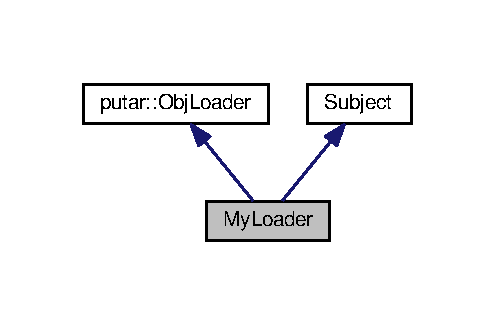
\includegraphics[width=238pt]{classMyLoader__inherit__graph}
\end{center}
\end{figure}


Collaboration diagram for My\+Loader\+:
\nopagebreak
\begin{figure}[H]
\begin{center}
\leavevmode
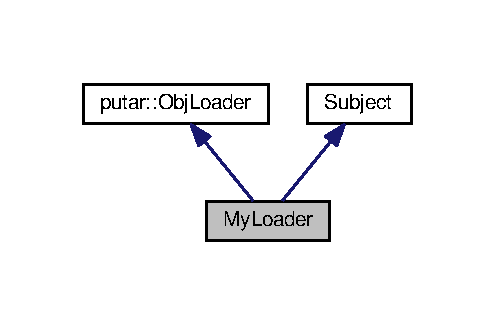
\includegraphics[width=238pt]{classMyLoader__coll__graph}
\end{center}
\end{figure}
\subsection*{Public Types}
\begin{DoxyCompactItemize}
\item 
typedef std\+::unique\+\_\+ptr$<$ \hyperlink{classMyLoader}{My\+Loader} $>$ \hyperlink{classMyLoader_acaf32066ff648b5d6743b91260c6ce28}{Ptr}\hypertarget{classMyLoader_acaf32066ff648b5d6743b91260c6ce28}{}\label{classMyLoader_acaf32066ff648b5d6743b91260c6ce28}

\begin{DoxyCompactList}\small\item\em Pointer. \end{DoxyCompactList}\end{DoxyCompactItemize}
\subsection*{Public Member Functions}
\begin{DoxyCompactItemize}
\item 
\hyperlink{classMyLoader_a40ebc4bfa57858e2cb1a7cdf8839a3da}{My\+Loader} (void)\hypertarget{classMyLoader_a40ebc4bfa57858e2cb1a7cdf8839a3da}{}\label{classMyLoader_a40ebc4bfa57858e2cb1a7cdf8839a3da}

\begin{DoxyCompactList}\small\item\em Construction. \end{DoxyCompactList}\item 
\hyperlink{classMyLoader_a9c6ce5cb2063955eace7a7fb8de0277b}{My\+Loader} (std\+::string config\+Filename)\hypertarget{classMyLoader_a9c6ce5cb2063955eace7a7fb8de0277b}{}\label{classMyLoader_a9c6ce5cb2063955eace7a7fb8de0277b}

\begin{DoxyCompactList}\small\item\em Construction. \end{DoxyCompactList}\item 
const std\+::string \& \hyperlink{classMyLoader_a10eb932a433ca5cd82258ba1c5da0291}{get\+Name} () const \hypertarget{classMyLoader_a10eb932a433ca5cd82258ba1c5da0291}{}\label{classMyLoader_a10eb932a433ca5cd82258ba1c5da0291}

\begin{DoxyCompactList}\small\item\em Name of the grabber. \end{DoxyCompactList}\item 
void \hyperlink{classMyLoader_a707d1e896cb08346acdfc43b42833422}{load\+Obj} ()\hypertarget{classMyLoader_a707d1e896cb08346acdfc43b42833422}{}\label{classMyLoader_a707d1e896cb08346acdfc43b42833422}

\begin{DoxyCompactList}\small\item\em Returns the current 2D image. \end{DoxyCompactList}\item 
void \hyperlink{classMyLoader_adfd8c3e638c7695ee086c5421670a747}{get\+Mesh} (\hyperlink{structputar_1_1obj__type}{obj\+\_\+type} \&p\+\_\+object) const \hypertarget{classMyLoader_adfd8c3e638c7695ee086c5421670a747}{}\label{classMyLoader_adfd8c3e638c7695ee086c5421670a747}

\begin{DoxyCompactList}\small\item\em Grab image and/or point cloud. \end{DoxyCompactList}\item 
void \hyperlink{classMyLoader_a6d01f2ecf0cd0167e37a55253ed3fdc2}{attach\+Visualizer} (\hyperlink{classQGLVisualizer}{Q\+G\+L\+Visualizer} $\ast$visualizer)\hypertarget{classMyLoader_a6d01f2ecf0cd0167e37a55253ed3fdc2}{}\label{classMyLoader_a6d01f2ecf0cd0167e37a55253ed3fdc2}

\begin{DoxyCompactList}\small\item\em Attach visualizer. \end{DoxyCompactList}\item 
void {\bfseries compute\+Mask} (const \hyperlink{namespaceputar_a8bf3c8025ae8f60f553a752014c9849a}{Mat34} camera\+Pose, cv\+::\+Mat \&mask)\hypertarget{classMyLoader_aefe8d1d90aa940353f8f794c4694277f}{}\label{classMyLoader_aefe8d1d90aa940353f8f794c4694277f}

\end{DoxyCompactItemize}
\subsection*{Additional Inherited Members}


\subsection{Detailed Description}
Obj\+Loader implementation. 

The documentation for this class was generated from the following file\+:\begin{DoxyCompactItemize}
\item 
Obj\+Loader/\hyperlink{MyLoader_8h}{My\+Loader.\+h}\end{DoxyCompactItemize}

\hypertarget{structputar_1_1obj__type}{}\section{putar\+:\+:obj\+\_\+type Struct Reference}
\label{structputar_1_1obj__type}\index{putar\+::obj\+\_\+type@{putar\+::obj\+\_\+type}}


Collaboration diagram for putar\+:\+:obj\+\_\+type\+:
\nopagebreak
\begin{figure}[H]
\begin{center}
\leavevmode
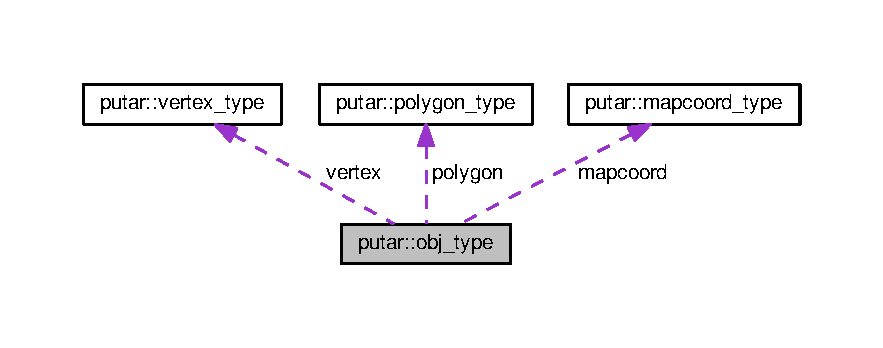
\includegraphics[width=350pt]{structputar_1_1obj__type__coll__graph}
\end{center}
\end{figure}
\subsection*{Public Attributes}
\begin{DoxyCompactItemize}
\item 
char {\bfseries name} \mbox{[}20\mbox{]}\hypertarget{structputar_1_1obj__type_acef3125ad5334ead5ebec173e8f0e2df}{}\label{structputar_1_1obj__type_acef3125ad5334ead5ebec173e8f0e2df}

\item 
int {\bfseries vertices\+\_\+qty}\hypertarget{structputar_1_1obj__type_a3356113c1689dc9acf2ab3e9eb2c9c30}{}\label{structputar_1_1obj__type_a3356113c1689dc9acf2ab3e9eb2c9c30}

\item 
int {\bfseries polygons\+\_\+qty}\hypertarget{structputar_1_1obj__type_ad6e2e366785cceba5a96c76b7676c918}{}\label{structputar_1_1obj__type_ad6e2e366785cceba5a96c76b7676c918}

\item 
\hyperlink{structputar_1_1vertex__type}{vertex\+\_\+type} {\bfseries vertex} \mbox{[}M\+A\+X\+\_\+\+V\+E\+R\+T\+I\+C\+ES\mbox{]}\hypertarget{structputar_1_1obj__type_a2c5d6f456a3bd2fae12bb23c15de7eca}{}\label{structputar_1_1obj__type_a2c5d6f456a3bd2fae12bb23c15de7eca}

\item 
\hyperlink{structputar_1_1polygon__type}{polygon\+\_\+type} {\bfseries polygon} \mbox{[}M\+A\+X\+\_\+\+P\+O\+L\+Y\+G\+O\+NS\mbox{]}\hypertarget{structputar_1_1obj__type_aeb6c3401f044e879c3c131de25d8c479}{}\label{structputar_1_1obj__type_aeb6c3401f044e879c3c131de25d8c479}

\item 
\hyperlink{structputar_1_1mapcoord__type}{mapcoord\+\_\+type} {\bfseries mapcoord} \mbox{[}M\+A\+X\+\_\+\+V\+E\+R\+T\+I\+C\+ES\mbox{]}\hypertarget{structputar_1_1obj__type_a65f52da561b9bc88146f8c2d06e44b99}{}\label{structputar_1_1obj__type_a65f52da561b9bc88146f8c2d06e44b99}

\item 
int {\bfseries id\+\_\+texture}\hypertarget{structputar_1_1obj__type_ac158c6ca2f665f7b549f954955002209}{}\label{structputar_1_1obj__type_ac158c6ca2f665f7b549f954955002209}

\end{DoxyCompactItemize}


The documentation for this struct was generated from the following file\+:\begin{DoxyCompactItemize}
\item 
Defs/\hyperlink{defs_8h}{defs.\+h}\end{DoxyCompactItemize}

\hypertarget{classputar_1_1Object3D}{}\section{putar\+:\+:Object3D Class Reference}
\label{classputar_1_1Object3D}\index{putar\+::\+Object3D@{putar\+::\+Object3D}}


3D object  




{\ttfamily \#include $<$defs.\+h$>$}

\subsection*{Public Types}
\begin{DoxyCompactItemize}
\item 
typedef std\+::vector$<$ \hyperlink{classputar_1_1Object3D}{Object3D} $>$ \hyperlink{classputar_1_1Object3D_a3cb755c7d5fbae630e1a188748cc9ba4}{Seq}\hypertarget{classputar_1_1Object3D_a3cb755c7d5fbae630e1a188748cc9ba4}{}\label{classputar_1_1Object3D_a3cb755c7d5fbae630e1a188748cc9ba4}

\begin{DoxyCompactList}\small\item\em set of nodes \end{DoxyCompactList}\end{DoxyCompactItemize}
\subsection*{Public Attributes}
\begin{DoxyCompactItemize}
\item 
std\+::vector$<$ \hyperlink{namespaceputar_a4c3cbb84a7c44d90796f404d9e2c10dc}{Vec3} $>$ \hyperlink{classputar_1_1Object3D_a98db9469ee89b49666fc0869534640dd}{vertices}\hypertarget{classputar_1_1Object3D_a98db9469ee89b49666fc0869534640dd}{}\label{classputar_1_1Object3D_a98db9469ee89b49666fc0869534640dd}

\begin{DoxyCompactList}\small\item\em vertices \end{DoxyCompactList}\item 
std\+::vector$<$ \hyperlink{namespaceputar_a4c3cbb84a7c44d90796f404d9e2c10dc}{Vec3} $>$ \hyperlink{classputar_1_1Object3D_abba256da57b53c6eee427645c75941fe}{uvs}\hypertarget{classputar_1_1Object3D_abba256da57b53c6eee427645c75941fe}{}\label{classputar_1_1Object3D_abba256da57b53c6eee427645c75941fe}

\begin{DoxyCompactList}\small\item\em texture coordinates \end{DoxyCompactList}\item 
std\+::vector$<$ \hyperlink{namespaceputar_a4c3cbb84a7c44d90796f404d9e2c10dc}{Vec3} $>$ \hyperlink{classputar_1_1Object3D_a1bba7733a918d59424e2fad741f6946a}{normals}\hypertarget{classputar_1_1Object3D_a1bba7733a918d59424e2fad741f6946a}{}\label{classputar_1_1Object3D_a1bba7733a918d59424e2fad741f6946a}

\begin{DoxyCompactList}\small\item\em normal vectors \end{DoxyCompactList}\end{DoxyCompactItemize}


\subsection{Detailed Description}
3D object 

The documentation for this class was generated from the following file\+:\begin{DoxyCompactItemize}
\item 
Defs/\hyperlink{defs_8h}{defs.\+h}\end{DoxyCompactItemize}

\hypertarget{classputar_1_1ObjLoader}{}\section{putar\+:\+:Obj\+Loader Class Reference}
\label{classputar_1_1ObjLoader}\index{putar\+::\+Obj\+Loader@{putar\+::\+Obj\+Loader}}


O\+B\+J\+L\+O\+A\+D\+ER interface.  




{\ttfamily \#include $<$obj\+Loader.\+h$>$}



Inheritance diagram for putar\+:\+:Obj\+Loader\+:
\nopagebreak
\begin{figure}[H]
\begin{center}
\leavevmode
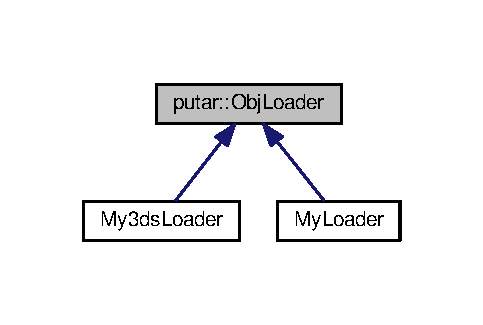
\includegraphics[width=232pt]{classputar_1_1ObjLoader__inherit__graph}
\end{center}
\end{figure}
\subsection*{Public Types}
\begin{DoxyCompactItemize}
\item 
enum \hyperlink{classputar_1_1ObjLoader_a4891ad8bb46a1414e2e9f202c1552e09}{Type} \{ \hyperlink{classputar_1_1ObjLoader_a4891ad8bb46a1414e2e9f202c1552e09aa774f269e111384506b37b5409932f3f}{T\+Y\+P\+E\+\_\+\+O\+BJ}, 
\hyperlink{classputar_1_1ObjLoader_a4891ad8bb46a1414e2e9f202c1552e09a484712937d79e778fdb8ee77a104087f}{T\+Y\+P\+E\+\_\+3\+DS}
 \}\begin{DoxyCompactList}\small\item\em \hyperlink{classputar_1_1ObjLoader}{Obj\+Loader} type. \end{DoxyCompactList}
\end{DoxyCompactItemize}
\subsection*{Public Member Functions}
\begin{DoxyCompactItemize}
\item 
\hyperlink{classputar_1_1ObjLoader_a6c20e772acf329b12f33759405070e36}{Obj\+Loader} (const std\+::string \+\_\+name, \hyperlink{classputar_1_1ObjLoader_a4891ad8bb46a1414e2e9f202c1552e09}{Type} \+\_\+type)\hypertarget{classputar_1_1ObjLoader_a6c20e772acf329b12f33759405070e36}{}\label{classputar_1_1ObjLoader_a6c20e772acf329b12f33759405070e36}

\begin{DoxyCompactList}\small\item\em overloaded constructor \end{DoxyCompactList}\item 
virtual const std\+::string \& \hyperlink{classputar_1_1ObjLoader_ae6dad14a43f50aa53290e98e0304a1b1}{get\+Name} () const =0\hypertarget{classputar_1_1ObjLoader_ae6dad14a43f50aa53290e98e0304a1b1}{}\label{classputar_1_1ObjLoader_ae6dad14a43f50aa53290e98e0304a1b1}

\begin{DoxyCompactList}\small\item\em Name of the grabber. \end{DoxyCompactList}\item 
virtual void \hyperlink{classputar_1_1ObjLoader_a28b81f23390667b1d7b6e56f8a7acc6d}{load\+Obj} ()=0\hypertarget{classputar_1_1ObjLoader_a28b81f23390667b1d7b6e56f8a7acc6d}{}\label{classputar_1_1ObjLoader_a28b81f23390667b1d7b6e56f8a7acc6d}

\begin{DoxyCompactList}\small\item\em Returns the current 2D image. \end{DoxyCompactList}\item 
virtual void \hyperlink{classputar_1_1ObjLoader_a3ea84cc9d21a2f35f6befc2cde1c3c80}{get\+Mesh} (\hyperlink{structputar_1_1obj__type}{obj\+\_\+type} \&p\+\_\+object) const =0\hypertarget{classputar_1_1ObjLoader_a3ea84cc9d21a2f35f6befc2cde1c3c80}{}\label{classputar_1_1ObjLoader_a3ea84cc9d21a2f35f6befc2cde1c3c80}

\begin{DoxyCompactList}\small\item\em Grab image and/or point cloud. \end{DoxyCompactList}\item 
virtual void {\bfseries compute\+Mask} (const \hyperlink{namespaceputar_a8bf3c8025ae8f60f553a752014c9849a}{Mat34} camera\+Pose, cv\+::\+Mat \&mask)=0\hypertarget{classputar_1_1ObjLoader_a098f9c13ea786f898110527517134a3b}{}\label{classputar_1_1ObjLoader_a098f9c13ea786f898110527517134a3b}

\item 
virtual void \hyperlink{classputar_1_1ObjLoader_a55c7bdde6fcfb844112428477b1dca23}{attach\+Visualizer} (\hyperlink{classQGLVisualizer}{Q\+G\+L\+Visualizer} $\ast$visualizer)=0\hypertarget{classputar_1_1ObjLoader_a55c7bdde6fcfb844112428477b1dca23}{}\label{classputar_1_1ObjLoader_a55c7bdde6fcfb844112428477b1dca23}

\begin{DoxyCompactList}\small\item\em Attach visualizer. \end{DoxyCompactList}\item 
virtual \hyperlink{classputar_1_1ObjLoader_a28de419299127b7e00aa25183a74f138}{$\sim$\+Obj\+Loader} ()\hypertarget{classputar_1_1ObjLoader_a28de419299127b7e00aa25183a74f138}{}\label{classputar_1_1ObjLoader_a28de419299127b7e00aa25183a74f138}

\begin{DoxyCompactList}\small\item\em Virtual descrutor. \end{DoxyCompactList}\end{DoxyCompactItemize}
\subsection*{Protected Attributes}
\begin{DoxyCompactItemize}
\item 
const std\+::string \hyperlink{classputar_1_1ObjLoader_ae4e76e742af0ec90329f1953dc9a129a}{name}\hypertarget{classputar_1_1ObjLoader_ae4e76e742af0ec90329f1953dc9a129a}{}\label{classputar_1_1ObjLoader_ae4e76e742af0ec90329f1953dc9a129a}

\begin{DoxyCompactList}\small\item\em Grabber name. \end{DoxyCompactList}\item 
\hyperlink{classputar_1_1ObjLoader_a4891ad8bb46a1414e2e9f202c1552e09}{Type} \hyperlink{classputar_1_1ObjLoader_a591a39e2a5203d9b76d00c41b0877016}{type}\hypertarget{classputar_1_1ObjLoader_a591a39e2a5203d9b76d00c41b0877016}{}\label{classputar_1_1ObjLoader_a591a39e2a5203d9b76d00c41b0877016}

\begin{DoxyCompactList}\small\item\em Grabber type. \end{DoxyCompactList}\end{DoxyCompactItemize}


\subsection{Detailed Description}
O\+B\+J\+L\+O\+A\+D\+ER interface. 

\subsection{Member Enumeration Documentation}
\index{putar\+::\+Obj\+Loader@{putar\+::\+Obj\+Loader}!Type@{Type}}
\index{Type@{Type}!putar\+::\+Obj\+Loader@{putar\+::\+Obj\+Loader}}
\subsubsection[{\texorpdfstring{Type}{Type}}]{\setlength{\rightskip}{0pt plus 5cm}enum {\bf putar\+::\+Obj\+Loader\+::\+Type}}\hypertarget{classputar_1_1ObjLoader_a4891ad8bb46a1414e2e9f202c1552e09}{}\label{classputar_1_1ObjLoader_a4891ad8bb46a1414e2e9f202c1552e09}


\hyperlink{classputar_1_1ObjLoader}{Obj\+Loader} type. 

\begin{Desc}
\item[Enumerator]\par
\begin{description}
\index{T\+Y\+P\+E\+\_\+\+O\+BJ@{T\+Y\+P\+E\+\_\+\+O\+BJ}!putar\+::\+Obj\+Loader@{putar\+::\+Obj\+Loader}}\index{putar\+::\+Obj\+Loader@{putar\+::\+Obj\+Loader}!T\+Y\+P\+E\+\_\+\+O\+BJ@{T\+Y\+P\+E\+\_\+\+O\+BJ}}\item[{\em 
T\+Y\+P\+E\+\_\+\+O\+BJ\hypertarget{classputar_1_1ObjLoader_a4891ad8bb46a1414e2e9f202c1552e09aa774f269e111384506b37b5409932f3f}{}\label{classputar_1_1ObjLoader_a4891ad8bb46a1414e2e9f202c1552e09aa774f269e111384506b37b5409932f3f}
}]O\+BJ camera. \index{T\+Y\+P\+E\+\_\+3\+DS@{T\+Y\+P\+E\+\_\+3\+DS}!putar\+::\+Obj\+Loader@{putar\+::\+Obj\+Loader}}\index{putar\+::\+Obj\+Loader@{putar\+::\+Obj\+Loader}!T\+Y\+P\+E\+\_\+3\+DS@{T\+Y\+P\+E\+\_\+3\+DS}}\item[{\em 
T\+Y\+P\+E\+\_\+3\+DS\hypertarget{classputar_1_1ObjLoader_a4891ad8bb46a1414e2e9f202c1552e09a484712937d79e778fdb8ee77a104087f}{}\label{classputar_1_1ObjLoader_a4891ad8bb46a1414e2e9f202c1552e09a484712937d79e778fdb8ee77a104087f}
}]3ds \end{description}
\end{Desc}


The documentation for this class was generated from the following file\+:\begin{DoxyCompactItemize}
\item 
Obj\+Loader/\hyperlink{objLoader_8h}{obj\+Loader.\+h}\end{DoxyCompactItemize}

\hypertarget{classObserver}{}\section{Observer Class Reference}
\label{classObserver}\index{Observer@{Observer}}


Inheritance diagram for Observer\+:
\nopagebreak
\begin{figure}[H]
\begin{center}
\leavevmode
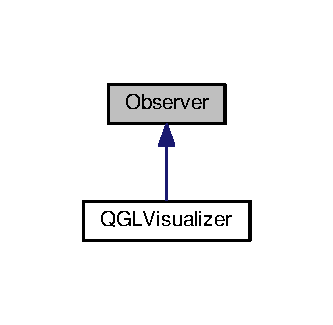
\includegraphics[width=160pt]{classObserver__inherit__graph}
\end{center}
\end{figure}
\subsection*{Public Member Functions}
\begin{DoxyCompactItemize}
\item 
virtual void {\bfseries update} (const \hyperlink{namespaceputar_a8bf3c8025ae8f60f553a752014c9849a}{putar\+::\+Mat34} \&object\+State)=0\hypertarget{classObserver_af8585a590e41dbffa1e53c7c98abe570}{}\label{classObserver_af8585a590e41dbffa1e53c7c98abe570}

\end{DoxyCompactItemize}


The documentation for this class was generated from the following file\+:\begin{DoxyCompactItemize}
\item 
Utilities/observer.\+h\end{DoxyCompactItemize}

\hypertarget{structputar_1_1polygon__type}{}\section{putar\+:\+:polygon\+\_\+type Struct Reference}
\label{structputar_1_1polygon__type}\index{putar\+::polygon\+\_\+type@{putar\+::polygon\+\_\+type}}
\subsection*{Public Attributes}
\begin{DoxyCompactItemize}
\item 
int {\bfseries a}\hypertarget{structputar_1_1polygon__type_ad21068ccb1eca6617cee793aa1f36616}{}\label{structputar_1_1polygon__type_ad21068ccb1eca6617cee793aa1f36616}

\item 
int {\bfseries b}\hypertarget{structputar_1_1polygon__type_a2900f8cfa5c7d03a811258756a2823a8}{}\label{structputar_1_1polygon__type_a2900f8cfa5c7d03a811258756a2823a8}

\item 
int {\bfseries c}\hypertarget{structputar_1_1polygon__type_aaff91e2352ece59b590e3cbdddc1a1df}{}\label{structputar_1_1polygon__type_aaff91e2352ece59b590e3cbdddc1a1df}

\end{DoxyCompactItemize}


The documentation for this struct was generated from the following file\+:\begin{DoxyCompactItemize}
\item 
Defs/\hyperlink{defs_8h}{defs.\+h}\end{DoxyCompactItemize}

\hypertarget{classQGLVisualizer}{}\section{Q\+G\+L\+Visualizer Class Reference}
\label{classQGLVisualizer}\index{Q\+G\+L\+Visualizer@{Q\+G\+L\+Visualizer}}


Map implementation.  




{\ttfamily \#include $<$Qvisualizer.\+h$>$}



Inheritance diagram for Q\+G\+L\+Visualizer\+:
\nopagebreak
\begin{figure}[H]
\begin{center}
\leavevmode
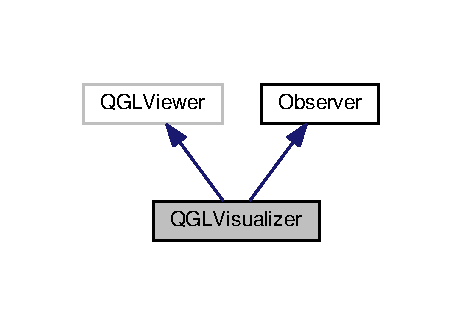
\includegraphics[width=222pt]{classQGLVisualizer__inherit__graph}
\end{center}
\end{figure}


Collaboration diagram for Q\+G\+L\+Visualizer\+:
\nopagebreak
\begin{figure}[H]
\begin{center}
\leavevmode
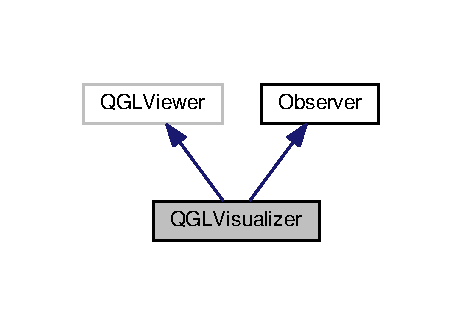
\includegraphics[width=222pt]{classQGLVisualizer__coll__graph}
\end{center}
\end{figure}
\subsection*{Classes}
\begin{DoxyCompactItemize}
\item 
class \hyperlink{classQGLVisualizer_1_1Config}{Config}
\end{DoxyCompactItemize}
\subsection*{Public Types}
\begin{DoxyCompactItemize}
\item 
typedef std\+::unique\+\_\+ptr$<$ \hyperlink{classQGLVisualizer}{Q\+G\+L\+Visualizer} $>$ \hyperlink{classQGLVisualizer_acc1cc199f42495cfda1df074ac06a57a}{Ptr}\hypertarget{classQGLVisualizer_acc1cc199f42495cfda1df074ac06a57a}{}\label{classQGLVisualizer_acc1cc199f42495cfda1df074ac06a57a}

\begin{DoxyCompactList}\small\item\em Pointer. \end{DoxyCompactList}\end{DoxyCompactItemize}
\subsection*{Public Member Functions}
\begin{DoxyCompactItemize}
\item 
\hyperlink{classQGLVisualizer_a7b1f8b4c0be357f9636d36ed47b09c0c}{Q\+G\+L\+Visualizer} (void)\hypertarget{classQGLVisualizer_a7b1f8b4c0be357f9636d36ed47b09c0c}{}\label{classQGLVisualizer_a7b1f8b4c0be357f9636d36ed47b09c0c}

\begin{DoxyCompactList}\small\item\em Construction. \end{DoxyCompactList}\item 
\hyperlink{classQGLVisualizer_adc2545fe51b3bfe3553b0031c8c66a31}{Q\+G\+L\+Visualizer} (std\+::string config\+Filename)\hypertarget{classQGLVisualizer_adc2545fe51b3bfe3553b0031c8c66a31}{}\label{classQGLVisualizer_adc2545fe51b3bfe3553b0031c8c66a31}

\begin{DoxyCompactList}\small\item\em Construction. \end{DoxyCompactList}\item 
void \hyperlink{classQGLVisualizer_a48d1c8965658c4e4bb1f5ead1b13adf7}{update} (const \hyperlink{namespaceputar_a8bf3c8025ae8f60f553a752014c9849a}{putar\+::\+Mat34} \&object\+State)\hypertarget{classQGLVisualizer_a48d1c8965658c4e4bb1f5ead1b13adf7}{}\label{classQGLVisualizer_a48d1c8965658c4e4bb1f5ead1b13adf7}

\begin{DoxyCompactList}\small\item\em update object state \end{DoxyCompactList}\item 
void \hyperlink{classQGLVisualizer_af264cd0d6ef16f7e1b45d9c7bd80196b}{update\+Mesh} (const \hyperlink{classputar_1_1Object3D}{Object3D} \&mesh)\hypertarget{classQGLVisualizer_af264cd0d6ef16f7e1b45d9c7bd80196b}{}\label{classQGLVisualizer_af264cd0d6ef16f7e1b45d9c7bd80196b}

\begin{DoxyCompactList}\small\item\em Updates mesh. \end{DoxyCompactList}\item 
void \hyperlink{classQGLVisualizer_ad88961c83066cb4b3874b7d4bb8419e0}{update\+Cloud} (cv\+::\+Mat R\+G\+BD)\hypertarget{classQGLVisualizer_ad88961c83066cb4b3874b7d4bb8419e0}{}\label{classQGLVisualizer_ad88961c83066cb4b3874b7d4bb8419e0}

\begin{DoxyCompactList}\small\item\em Updates cloud. \end{DoxyCompactList}\item 
\hyperlink{classQGLVisualizer_a7ad8fe9531404411e1bc908f7d07edc0}{$\sim$\+Q\+G\+L\+Visualizer} (void)\hypertarget{classQGLVisualizer_a7ad8fe9531404411e1bc908f7d07edc0}{}\label{classQGLVisualizer_a7ad8fe9531404411e1bc908f7d07edc0}

\begin{DoxyCompactList}\small\item\em Destruction. \end{DoxyCompactList}\end{DoxyCompactItemize}


\subsection{Detailed Description}
Map implementation. 

The documentation for this class was generated from the following file\+:\begin{DoxyCompactItemize}
\item 
Visualizer/Qvisualizer.\+h\end{DoxyCompactItemize}

\hypertarget{classStopwatch}{}\section{Stopwatch$<$ TimeT, ClockT, DurationT $>$ Class Template Reference}
\label{classStopwatch}\index{Stopwatch$<$ Time\+T, Clock\+T, Duration\+T $>$@{Stopwatch$<$ Time\+T, Clock\+T, Duration\+T $>$}}
\subsection*{Public Member Functions}
\begin{DoxyCompactItemize}
\item 
void {\bfseries start} ()\hypertarget{classStopwatch_a9e2f8235b8ff4047283dab800d3099fa}{}\label{classStopwatch_a9e2f8235b8ff4047283dab800d3099fa}

\item 
DurationT {\bfseries stop} ()\hypertarget{classStopwatch_a9a935a68524f7768c990eab9090e96ba}{}\label{classStopwatch_a9a935a68524f7768c990eab9090e96ba}

\item 
DurationT {\bfseries elapsed} ()\hypertarget{classStopwatch_a4dc9e5e83bcb010caaacffb98f29674a}{}\label{classStopwatch_a4dc9e5e83bcb010caaacffb98f29674a}

\end{DoxyCompactItemize}


The documentation for this class was generated from the following file\+:\begin{DoxyCompactItemize}
\item 
Utilities/stopwatch.\+h\end{DoxyCompactItemize}

\hypertarget{classSubject}{}\section{Subject Class Reference}
\label{classSubject}\index{Subject@{Subject}}


Inheritance diagram for Subject\+:
\nopagebreak
\begin{figure}[H]
\begin{center}
\leavevmode
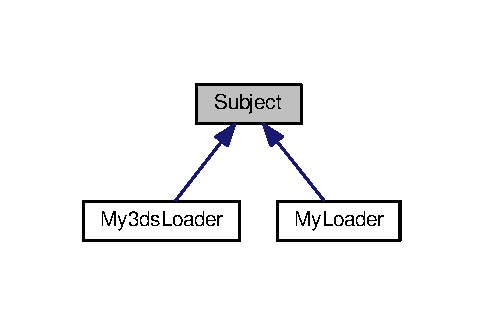
\includegraphics[width=232pt]{classSubject__inherit__graph}
\end{center}
\end{figure}
\subsection*{Public Member Functions}
\begin{DoxyCompactItemize}
\item 
void {\bfseries attach} (\hyperlink{classObserver}{Observer} $\ast$observer)\hypertarget{classSubject_a0884bfe374d352c6488a1e40c84246c8}{}\label{classSubject_a0884bfe374d352c6488a1e40c84246c8}

\item 
void {\bfseries detach} (\hyperlink{classObserver}{Observer} $\ast$observer)\hypertarget{classSubject_a752a7596d52ab986539232f8377ca92c}{}\label{classSubject_a752a7596d52ab986539232f8377ca92c}

\item 
void {\bfseries notify} (const \hyperlink{namespaceputar_a8bf3c8025ae8f60f553a752014c9849a}{putar\+::\+Mat34} \&object\+State)\hypertarget{classSubject_a7776ffd834c150b7e326489c69497e00}{}\label{classSubject_a7776ffd834c150b7e326489c69497e00}

\end{DoxyCompactItemize}


The documentation for this class was generated from the following file\+:\begin{DoxyCompactItemize}
\item 
Utilities/observer.\+h\end{DoxyCompactItemize}

\hypertarget{structputar_1_1vertex__type}{}\section{putar\+:\+:vertex\+\_\+type Struct Reference}
\label{structputar_1_1vertex__type}\index{putar\+::vertex\+\_\+type@{putar\+::vertex\+\_\+type}}
\subsection*{Public Attributes}
\begin{DoxyCompactItemize}
\item 
float {\bfseries x}\hypertarget{structputar_1_1vertex__type_a552b7fb64487621f35436eb70981e1b7}{}\label{structputar_1_1vertex__type_a552b7fb64487621f35436eb70981e1b7}

\item 
float {\bfseries y}\hypertarget{structputar_1_1vertex__type_a798b0972222fb9a6c69a6d32b1adee8c}{}\label{structputar_1_1vertex__type_a798b0972222fb9a6c69a6d32b1adee8c}

\item 
float {\bfseries z}\hypertarget{structputar_1_1vertex__type_a04b2f453fb5b6f9f9d987a1bd3c9f36d}{}\label{structputar_1_1vertex__type_a04b2f453fb5b6f9f9d987a1bd3c9f36d}

\end{DoxyCompactItemize}


The documentation for this struct was generated from the following file\+:\begin{DoxyCompactItemize}
\item 
Defs/\hyperlink{defs_8h}{defs.\+h}\end{DoxyCompactItemize}

\chapter{File Documentation}
\hypertarget{defs_8h}{}\section{Defs/defs.h File Reference}
\label{defs_8h}\index{Defs/defs.\+h@{Defs/defs.\+h}}
{\ttfamily \#include $<$cstdint$>$}\\*
{\ttfamily \#include $<$vector$>$}\\*
{\ttfamily \#include $<$memory$>$}\\*
{\ttfamily \#include $<$cmath$>$}\\*
{\ttfamily \#include \char`\"{}opencv\+Core.\+h\char`\"{}}\\*
{\ttfamily \#include \char`\"{}eigen3.\+h\char`\"{}}\\*
Include dependency graph for defs.\+h\+:
\nopagebreak
\begin{figure}[H]
\begin{center}
\leavevmode
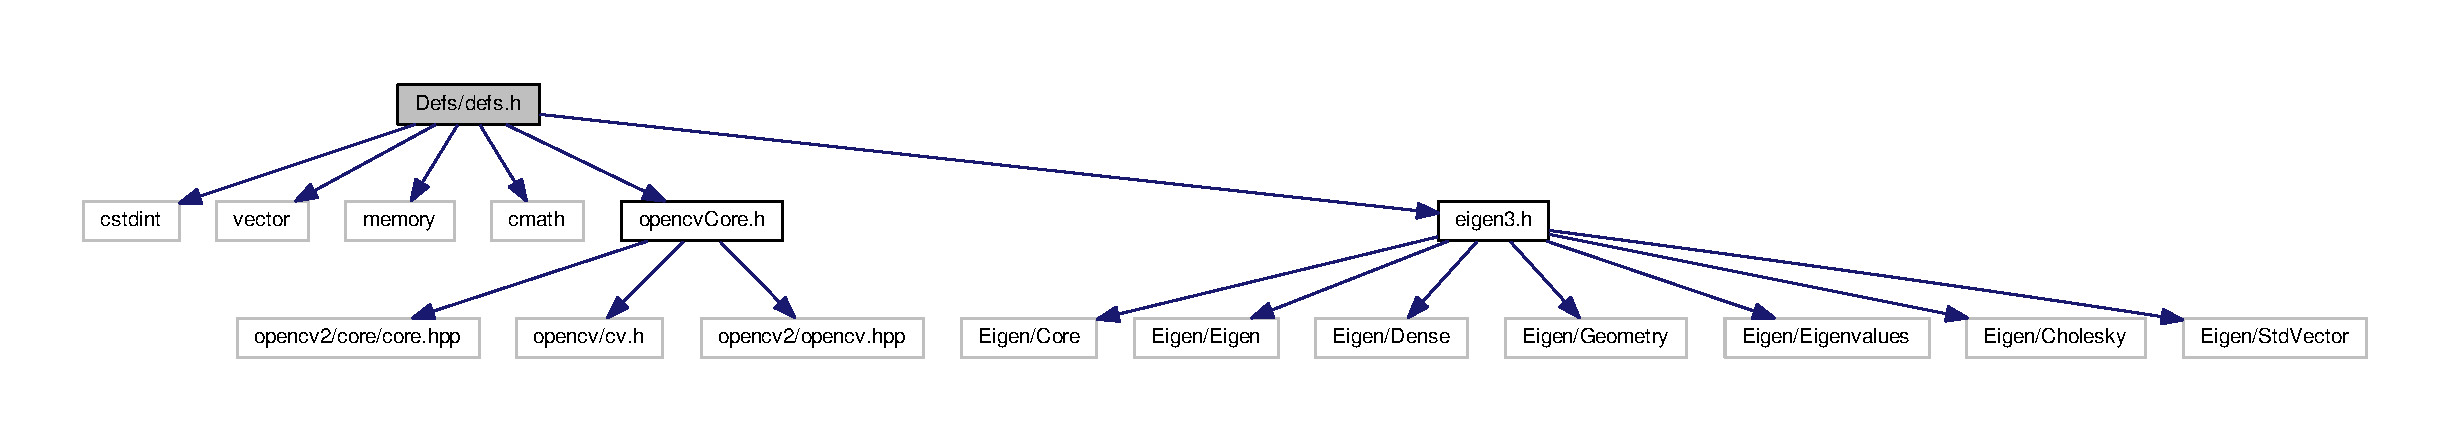
\includegraphics[width=350pt]{defs_8h__incl}
\end{center}
\end{figure}
This graph shows which files directly or indirectly include this file\+:
\nopagebreak
\begin{figure}[H]
\begin{center}
\leavevmode
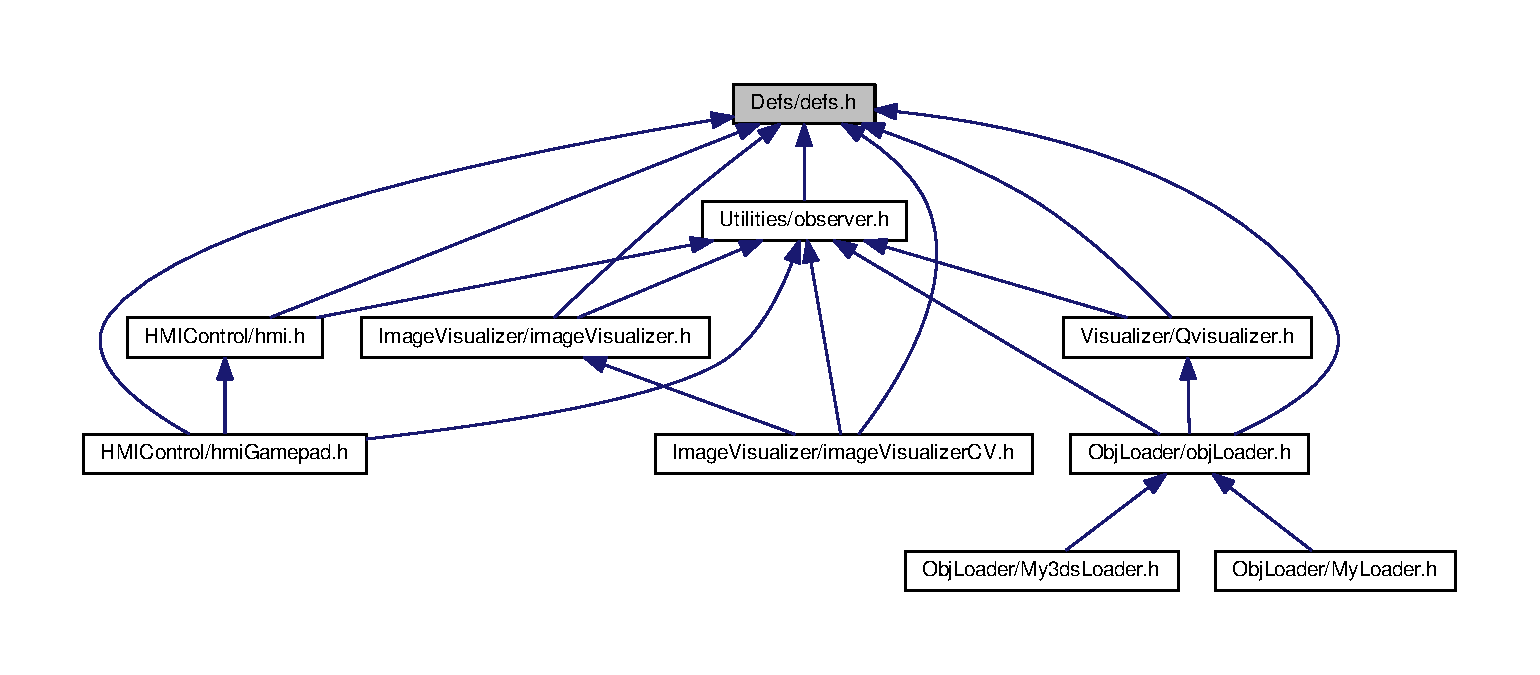
\includegraphics[width=350pt]{defs_8h__dep__incl}
\end{center}
\end{figure}
\subsection*{Classes}
\begin{DoxyCompactItemize}
\item 
struct \hyperlink{structputar_1_1vertex__type}{putar\+::vertex\+\_\+type}
\item 
struct \hyperlink{structputar_1_1polygon__type}{putar\+::polygon\+\_\+type}
\item 
struct \hyperlink{structputar_1_1mapcoord__type}{putar\+::mapcoord\+\_\+type}
\item 
struct \hyperlink{structputar_1_1obj__type}{putar\+::obj\+\_\+type}
\item 
class \hyperlink{classputar_1_1Object3D}{putar\+::\+Object3D}
\begin{DoxyCompactList}\small\item\em 3D object \end{DoxyCompactList}\end{DoxyCompactItemize}
\subsection*{Namespaces}
\begin{DoxyCompactItemize}
\item 
 \hyperlink{namespaceputar}{putar}
\begin{DoxyCompactList}\small\item\em putslam name space \end{DoxyCompactList}\end{DoxyCompactItemize}
\subsection*{Macros}
\begin{DoxyCompactItemize}
\item 
\#define {\bfseries M\+A\+X\+\_\+\+V\+E\+R\+T\+I\+C\+ES}~8000\hypertarget{defs_8h_a0fdb7b933ef091574ff57d1f36dd4167}{}\label{defs_8h_a0fdb7b933ef091574ff57d1f36dd4167}

\item 
\#define {\bfseries M\+A\+X\+\_\+\+P\+O\+L\+Y\+G\+O\+NS}~8000\hypertarget{defs_8h_a0aaa578e910c66db37a344dcfc514f3b}{}\label{defs_8h_a0aaa578e910c66db37a344dcfc514f3b}

\end{DoxyCompactItemize}
\subsection*{Typedefs}
\begin{DoxyCompactItemize}
\item 
typedef Eigen\+::\+Translation$<$ double, 3 $>$ \hyperlink{namespaceputar_a4c3cbb84a7c44d90796f404d9e2c10dc}{putar\+::\+Vec3}\hypertarget{namespaceputar_a4c3cbb84a7c44d90796f404d9e2c10dc}{}\label{namespaceputar_a4c3cbb84a7c44d90796f404d9e2c10dc}

\begin{DoxyCompactList}\small\item\em 3 element vector class \end{DoxyCompactList}\item 
typedef Eigen\+::\+Matrix$<$ double, 3, 3 $>$ \hyperlink{namespaceputar_aee57be2241e98d794717b88483857084}{putar\+::\+Mat33}\hypertarget{namespaceputar_aee57be2241e98d794717b88483857084}{}\label{namespaceputar_aee57be2241e98d794717b88483857084}

\begin{DoxyCompactList}\small\item\em Matrix representation of S\+O(3) group of rotations. \end{DoxyCompactList}\item 
typedef Eigen\+::\+Quaternion$<$ double $>$ \hyperlink{namespaceputar_a80c20cdfaa95579ce0f4eaf85f609e31}{putar\+::\+Quaternion}\hypertarget{namespaceputar_a80c20cdfaa95579ce0f4eaf85f609e31}{}\label{namespaceputar_a80c20cdfaa95579ce0f4eaf85f609e31}

\begin{DoxyCompactList}\small\item\em Quaternion representation of S\+O(3) group of rotations. \end{DoxyCompactList}\item 
typedef Eigen\+::\+Transform$<$ double, 3, Eigen\+::\+Affine $>$ \hyperlink{namespaceputar_a8bf3c8025ae8f60f553a752014c9849a}{putar\+::\+Mat34}\hypertarget{namespaceputar_a8bf3c8025ae8f60f553a752014c9849a}{}\label{namespaceputar_a8bf3c8025ae8f60f553a752014c9849a}

\begin{DoxyCompactList}\small\item\em Homogeneous representation of S\+E(3) rigid body transformations. \end{DoxyCompactList}\item 
typedef cv\+::\+Mat \hyperlink{namespaceputar_a6b914df3faf7862e1bd631536309251a}{putar\+::\+Image}\hypertarget{namespaceputar_a6b914df3faf7862e1bd631536309251a}{}\label{namespaceputar_a6b914df3faf7862e1bd631536309251a}

\begin{DoxyCompactList}\small\item\em Image. \end{DoxyCompactList}\item 
typedef struct \hyperlink{structputar_1_1obj__type}{putar\+::obj\+\_\+type} $\ast$ {\bfseries putar\+::obj\+\_\+type\+\_\+ptr}\hypertarget{namespaceputar_a5c44aa91da318ae2ead9456c2f2de2ac}{}\label{namespaceputar_a5c44aa91da318ae2ead9456c2f2de2ac}

\end{DoxyCompactItemize}


\subsection{Detailed Description}
Simulator definitions 
\hypertarget{hmi_8h}{}\section{H\+M\+I\+Control/hmi.h File Reference}
\label{hmi_8h}\index{H\+M\+I\+Control/hmi.\+h@{H\+M\+I\+Control/hmi.\+h}}
{\ttfamily \#include \char`\"{}../\+Defs/defs.\+h\char`\"{}}\\*
{\ttfamily \#include \char`\"{}Utilities/observer.\+h\char`\"{}}\\*
{\ttfamily \#include $<$iostream$>$}\\*
{\ttfamily \#include $<$string$>$}\\*
Include dependency graph for hmi.\+h\+:
\nopagebreak
\begin{figure}[H]
\begin{center}
\leavevmode
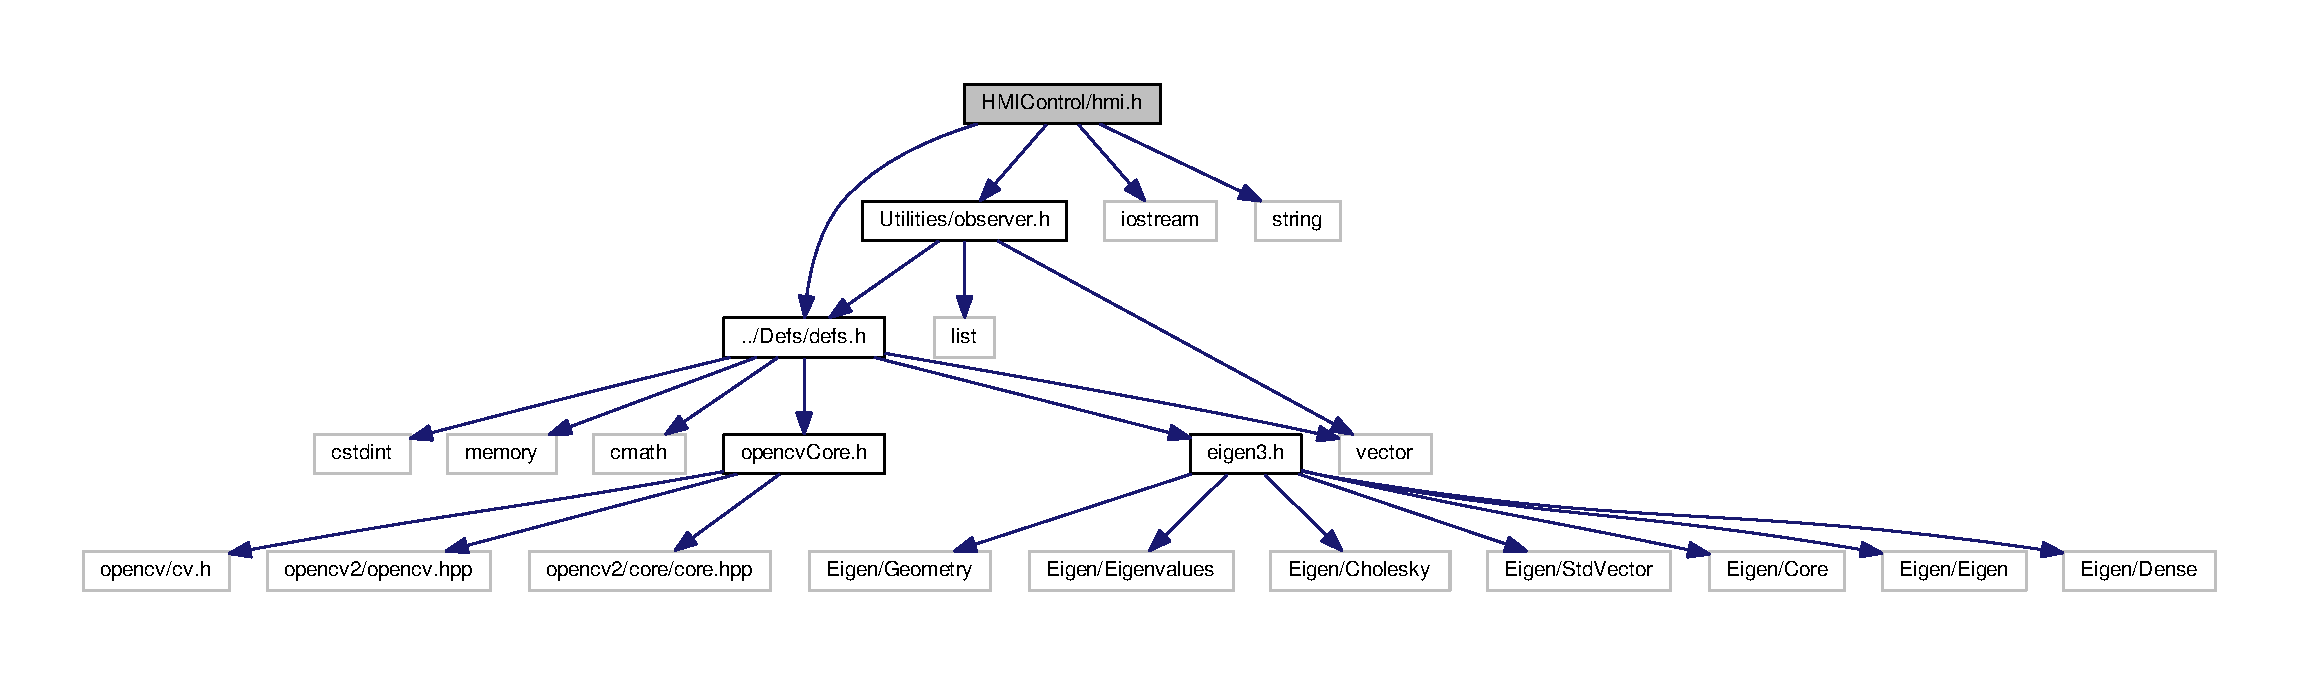
\includegraphics[width=350pt]{hmi_8h__incl}
\end{center}
\end{figure}
This graph shows which files directly or indirectly include this file\+:
\nopagebreak
\begin{figure}[H]
\begin{center}
\leavevmode
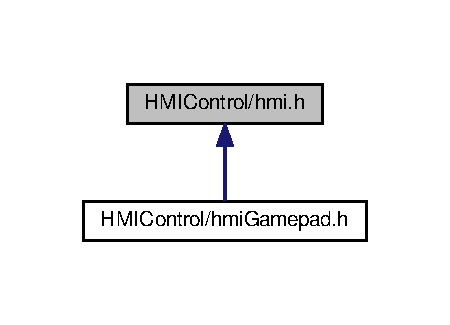
\includegraphics[width=216pt]{hmi_8h__dep__incl}
\end{center}
\end{figure}
\subsection*{Classes}
\begin{DoxyCompactItemize}
\item 
class \hyperlink{classputar_1_1Hmi}{putar\+::\+Hmi}
\end{DoxyCompactItemize}
\subsection*{Namespaces}
\begin{DoxyCompactItemize}
\item 
 \hyperlink{namespaceputar}{putar}
\begin{DoxyCompactList}\small\item\em putslam name space \end{DoxyCompactList}\end{DoxyCompactItemize}


\subsection{Detailed Description}
hmi interface 
\hypertarget{My3dsLoader_8h}{}\section{Obj\+Loader/\+My3ds\+Loader.h File Reference}
\label{My3dsLoader_8h}\index{Obj\+Loader/\+My3ds\+Loader.\+h@{Obj\+Loader/\+My3ds\+Loader.\+h}}
{\ttfamily \#include \char`\"{}obj\+Loader.\+h\char`\"{}}\\*
{\ttfamily \#include \char`\"{}../../3rd\+Party/tiny\+X\+M\+L/tinyxml2.\+h\char`\"{}}\\*
{\ttfamily \#include $<$iostream$>$}\\*
{\ttfamily \#include $<$memory$>$}\\*
{\ttfamily \#include $<$sys/stat.\+h$>$}\\*
Include dependency graph for My3ds\+Loader.\+h\+:
\nopagebreak
\begin{figure}[H]
\begin{center}
\leavevmode
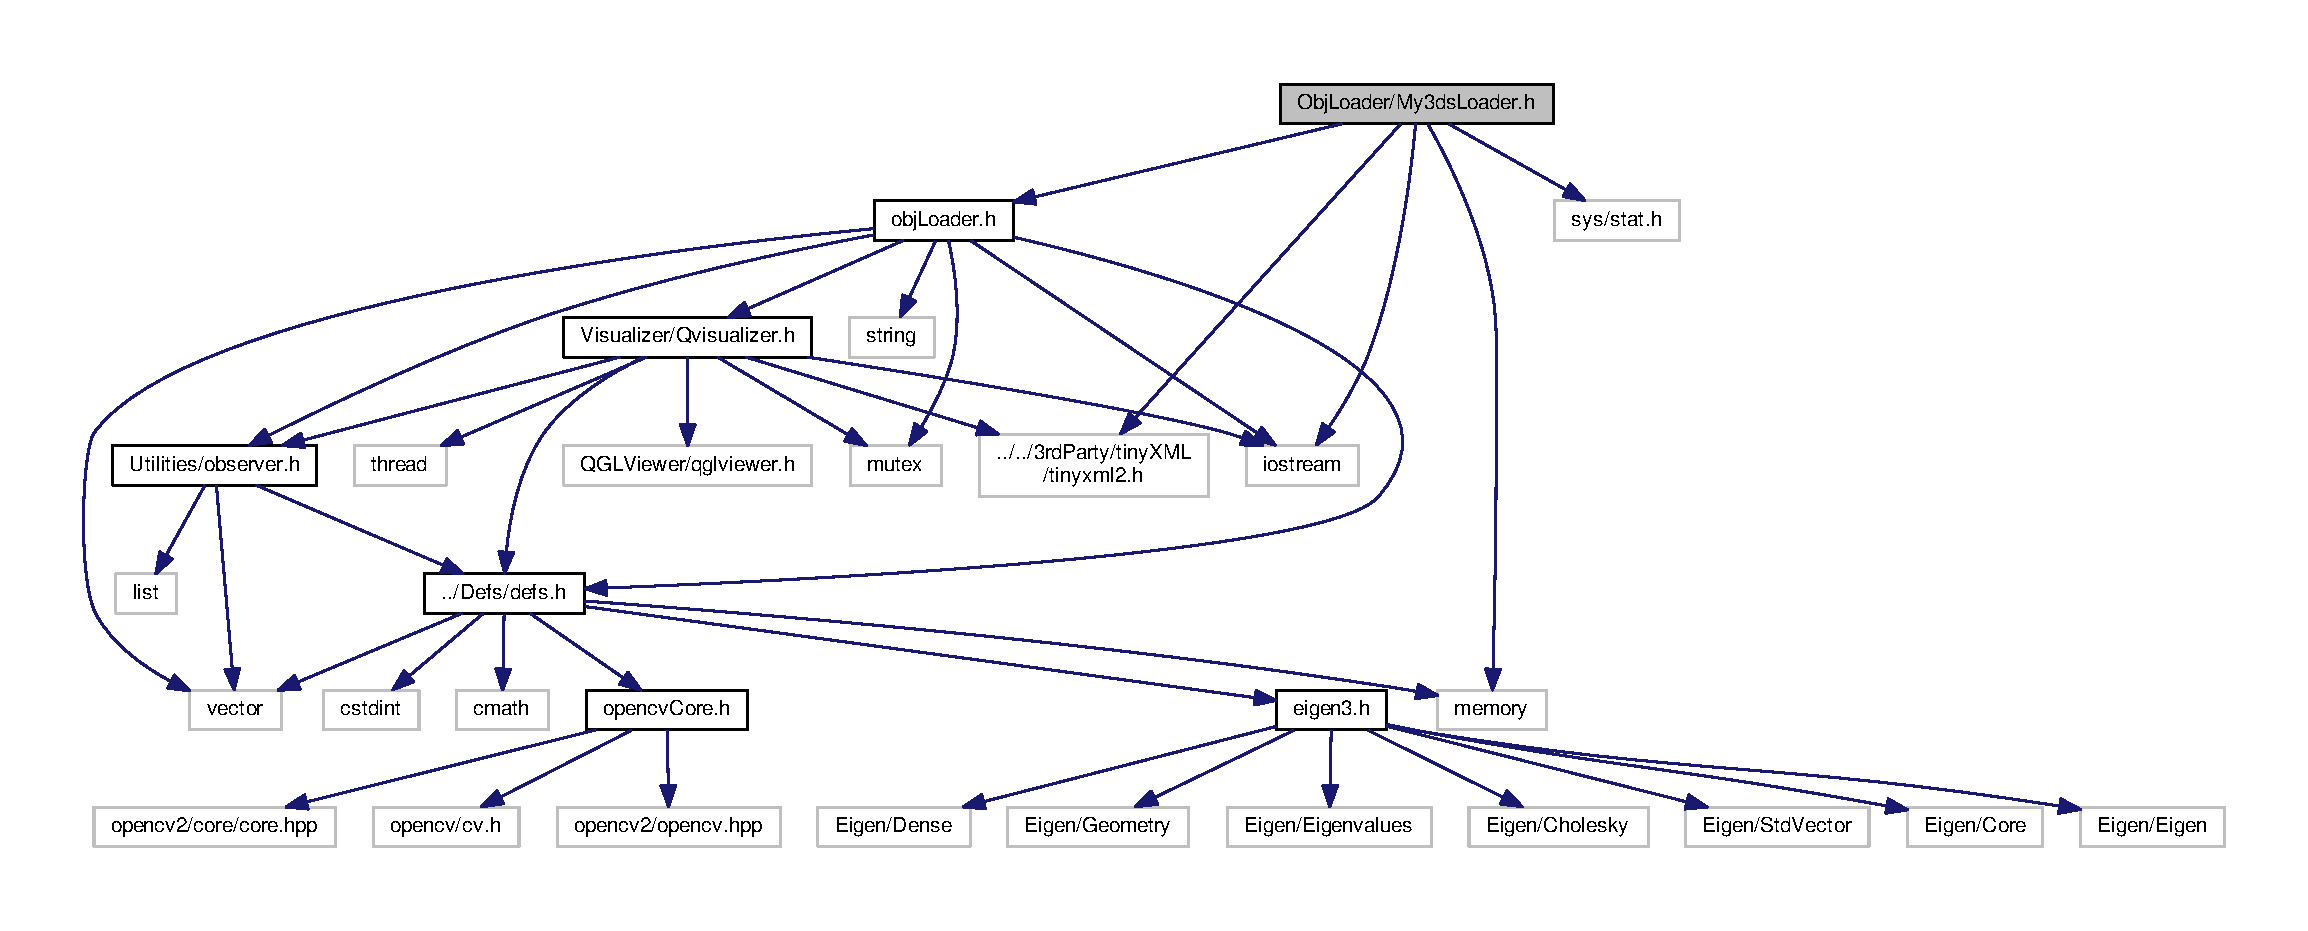
\includegraphics[width=350pt]{My3dsLoader_8h__incl}
\end{center}
\end{figure}
\subsection*{Classes}
\begin{DoxyCompactItemize}
\item 
class \hyperlink{classMy3dsLoader}{My3ds\+Loader}
\begin{DoxyCompactList}\small\item\em Obj\+Loader implementation. \end{DoxyCompactList}\end{DoxyCompactItemize}
\subsection*{Namespaces}
\begin{DoxyCompactItemize}
\item 
 \hyperlink{namespaceputar}{putar}
\begin{DoxyCompactList}\small\item\em putslam name space \end{DoxyCompactList}\end{DoxyCompactItemize}
\subsection*{Functions}
\begin{DoxyCompactItemize}
\item 
\hyperlink{classputar_1_1ObjLoader}{Obj\+Loader} $\ast$ \hyperlink{namespaceputar_a6b76c4a83de676f506ccfb24399705fb}{putar\+::create\+My3ds\+Loader} (void)\hypertarget{namespaceputar_a6b76c4a83de676f506ccfb24399705fb}{}\label{namespaceputar_a6b76c4a83de676f506ccfb24399705fb}

\begin{DoxyCompactList}\small\item\em create a single \hyperlink{classputar_1_1ObjLoader}{Obj\+Loader} \end{DoxyCompactList}\item 
\hyperlink{classputar_1_1ObjLoader}{Obj\+Loader} $\ast$ {\bfseries putar\+::create\+My3ds\+Loader} (std\+::string config\+File)\hypertarget{namespaceputar_a631859f4fce1b129afd30aa34b54b728}{}\label{namespaceputar_a631859f4fce1b129afd30aa34b54b728}

\end{DoxyCompactItemize}


\subsection{Detailed Description}
implementation -\/ My 3\+DS Loader 
\hypertarget{MyLoader_8h}{}\section{Obj\+Loader/\+My\+Loader.h File Reference}
\label{MyLoader_8h}\index{Obj\+Loader/\+My\+Loader.\+h@{Obj\+Loader/\+My\+Loader.\+h}}
{\ttfamily \#include \char`\"{}obj\+Loader.\+h\char`\"{}}\\*
{\ttfamily \#include \char`\"{}../../3rd\+Party/tiny\+X\+M\+L/tinyxml2.\+h\char`\"{}}\\*
{\ttfamily \#include $<$iostream$>$}\\*
{\ttfamily \#include $<$memory$>$}\\*
Include dependency graph for My\+Loader.\+h\+:
\nopagebreak
\begin{figure}[H]
\begin{center}
\leavevmode
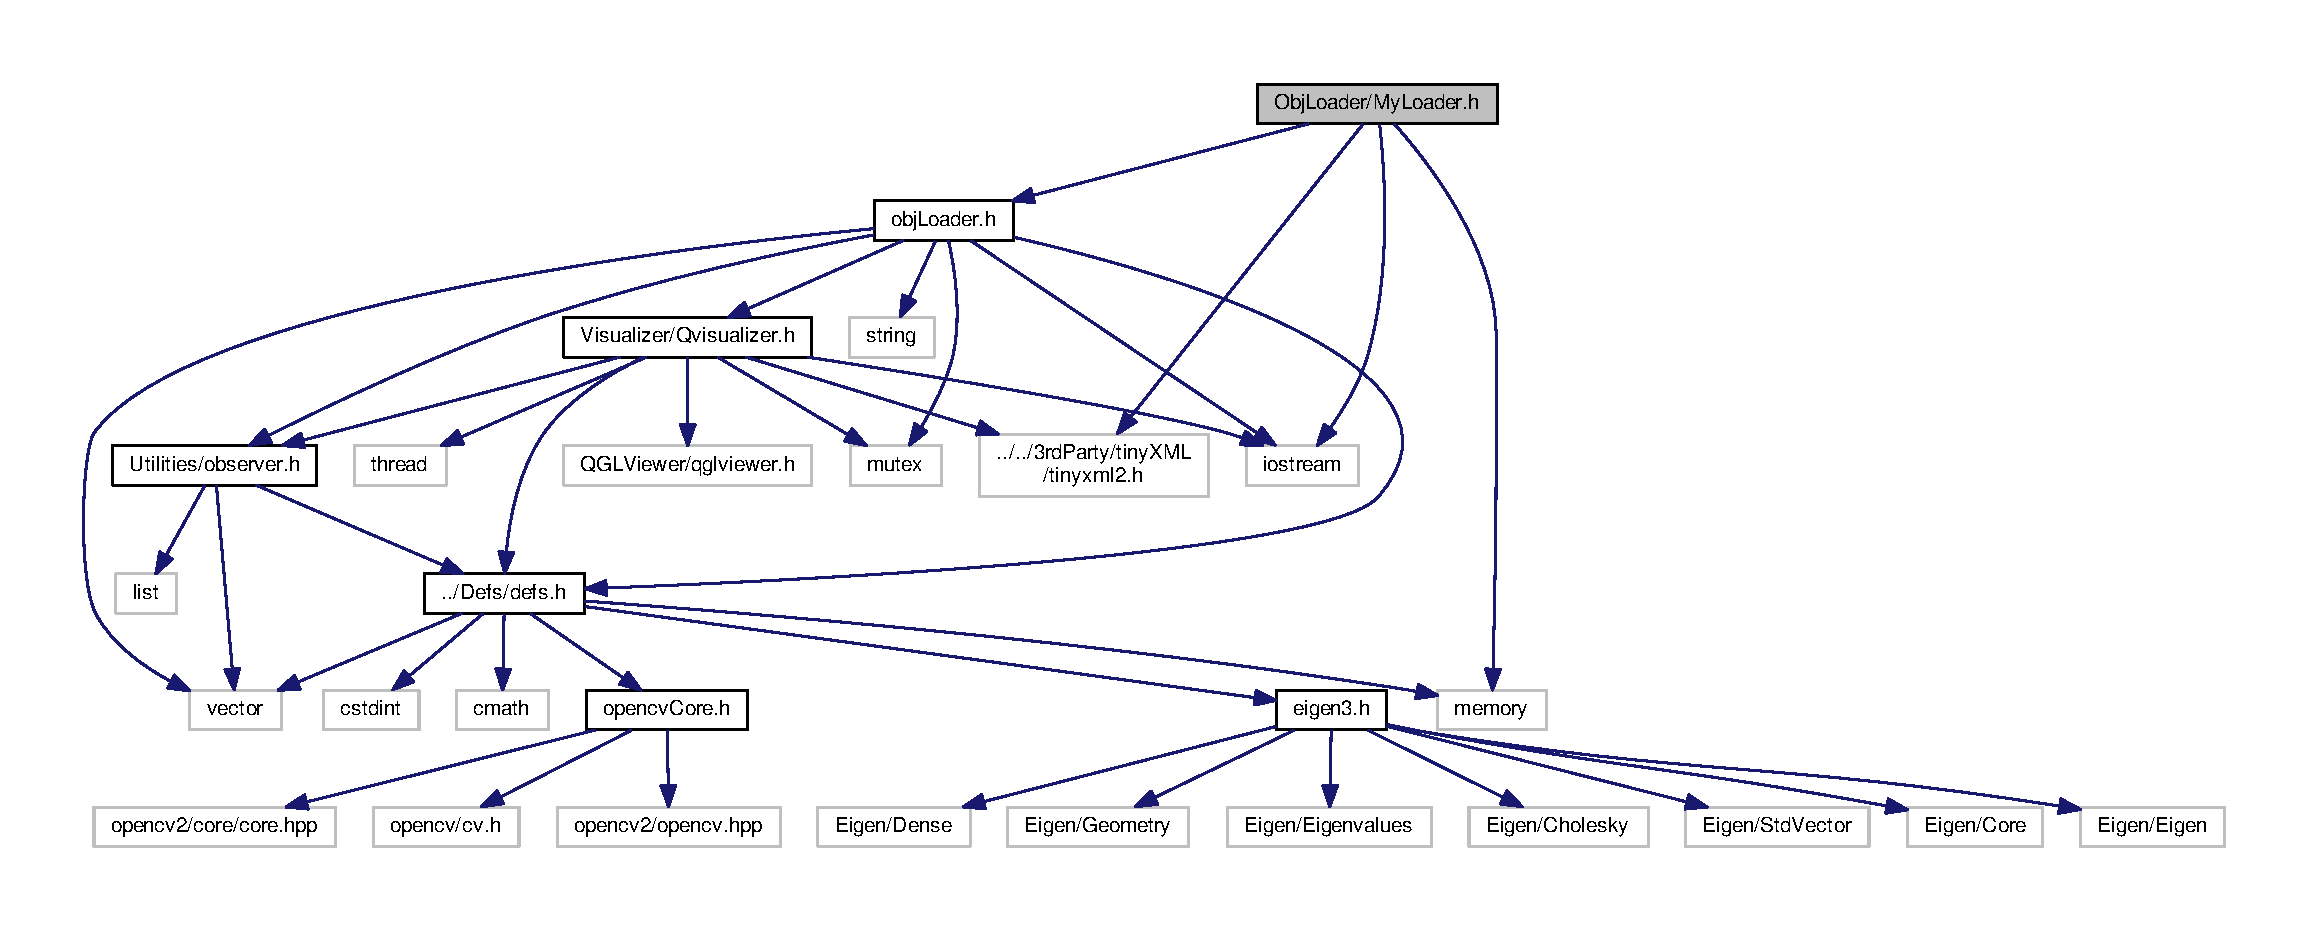
\includegraphics[width=350pt]{MyLoader_8h__incl}
\end{center}
\end{figure}
\subsection*{Classes}
\begin{DoxyCompactItemize}
\item 
class \hyperlink{classMyLoader}{My\+Loader}
\begin{DoxyCompactList}\small\item\em Obj\+Loader implementation. \end{DoxyCompactList}\end{DoxyCompactItemize}
\subsection*{Namespaces}
\begin{DoxyCompactItemize}
\item 
 \hyperlink{namespaceputar}{putar}
\begin{DoxyCompactList}\small\item\em putslam name space \end{DoxyCompactList}\end{DoxyCompactItemize}
\subsection*{Functions}
\begin{DoxyCompactItemize}
\item 
\hyperlink{classputar_1_1ObjLoader}{Obj\+Loader} $\ast$ \hyperlink{namespaceputar_ad2bde0bc3257e7e3e2d8c2fa6311d42d}{putar\+::create\+My\+Loader} (void)\hypertarget{namespaceputar_ad2bde0bc3257e7e3e2d8c2fa6311d42d}{}\label{namespaceputar_ad2bde0bc3257e7e3e2d8c2fa6311d42d}

\begin{DoxyCompactList}\small\item\em create a single \hyperlink{classputar_1_1ObjLoader}{Obj\+Loader} \end{DoxyCompactList}\item 
\hyperlink{classputar_1_1ObjLoader}{Obj\+Loader} $\ast$ {\bfseries putar\+::create\+My\+Loader} (std\+::string config\+File)\hypertarget{namespaceputar_afcf7f746d647ed671ab7d8c0cb06e528}{}\label{namespaceputar_afcf7f746d647ed671ab7d8c0cb06e528}

\end{DoxyCompactItemize}


\subsection{Detailed Description}
implementation -\/ My Loader 
\hypertarget{objLoader_8h}{}\section{Obj\+Loader/obj\+Loader.h File Reference}
\label{objLoader_8h}\index{Obj\+Loader/obj\+Loader.\+h@{Obj\+Loader/obj\+Loader.\+h}}
{\ttfamily \#include \char`\"{}../\+Defs/defs.\+h\char`\"{}}\\*
{\ttfamily \#include \char`\"{}Utilities/observer.\+h\char`\"{}}\\*
{\ttfamily \#include \char`\"{}Visualizer/\+Qvisualizer.\+h\char`\"{}}\\*
{\ttfamily \#include $<$iostream$>$}\\*
{\ttfamily \#include $<$string$>$}\\*
{\ttfamily \#include $<$vector$>$}\\*
{\ttfamily \#include $<$mutex$>$}\\*
Include dependency graph for obj\+Loader.\+h\+:
\nopagebreak
\begin{figure}[H]
\begin{center}
\leavevmode
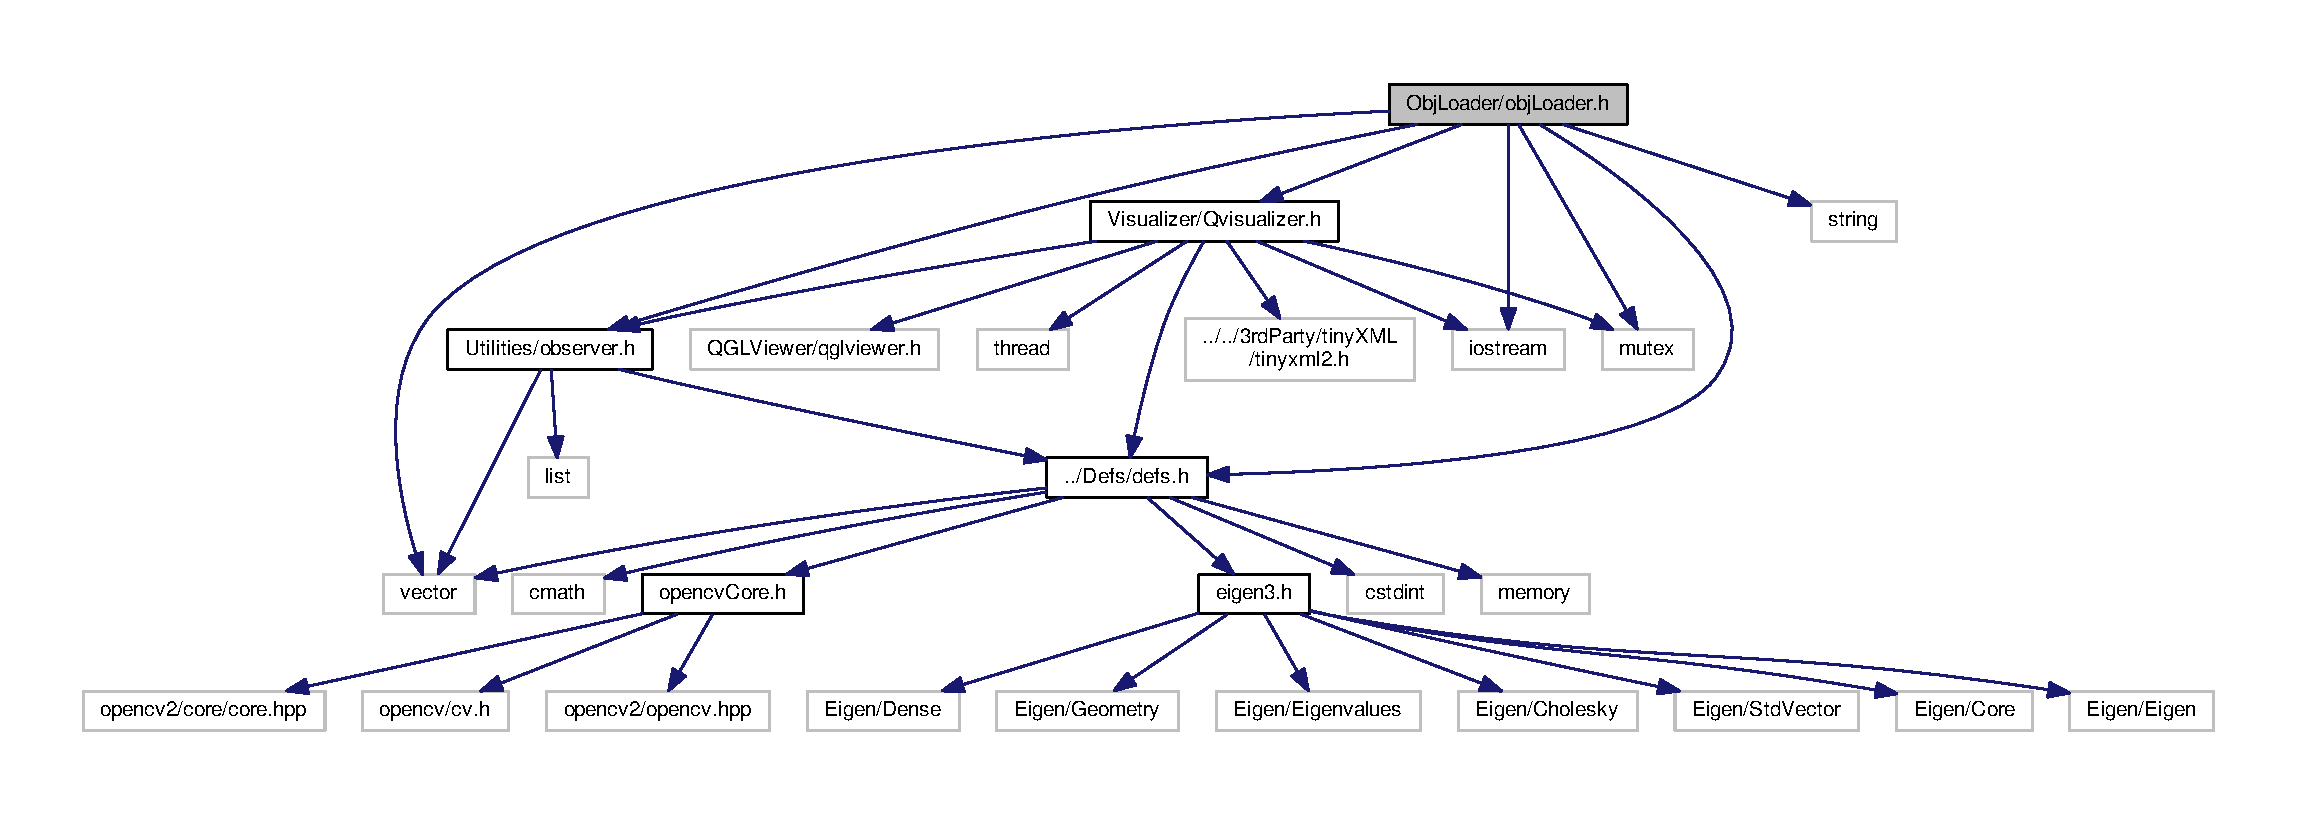
\includegraphics[width=350pt]{objLoader_8h__incl}
\end{center}
\end{figure}
This graph shows which files directly or indirectly include this file\+:
\nopagebreak
\begin{figure}[H]
\begin{center}
\leavevmode
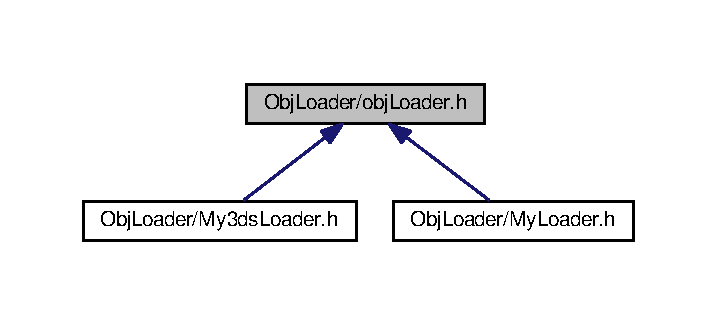
\includegraphics[width=344pt]{objLoader_8h__dep__incl}
\end{center}
\end{figure}
\subsection*{Classes}
\begin{DoxyCompactItemize}
\item 
class \hyperlink{classputar_1_1ObjLoader}{putar\+::\+Obj\+Loader}
\begin{DoxyCompactList}\small\item\em O\+B\+J\+L\+O\+A\+D\+ER interface. \end{DoxyCompactList}\end{DoxyCompactItemize}
\subsection*{Namespaces}
\begin{DoxyCompactItemize}
\item 
 \hyperlink{namespaceputar}{putar}
\begin{DoxyCompactList}\small\item\em putslam name space \end{DoxyCompactList}\end{DoxyCompactItemize}


\subsection{Detailed Description}
Obj Loade interface 
%--- End generated contents ---

% Index
\backmatter
\newpage
\phantomsection
\clearemptydoublepage
\addcontentsline{toc}{chapter}{Index}
\printindex

\end{document}
